\section{Grafische Benutzeroberfläche (Website)}
%\chapter{Website / front end}
Die bisherige Anzeige der Wetterdaten basiert auf Adobe Flash, was nicht von allen Browsern unterstützt wird (siehe Fachmodul-Bericht). Die neue (2014) HTML5-Spezifikation ermöglicht es dynamische Grafiken zu erzeugen, die nativ von allen Web-Browsern dargestellt werden können.



%% ############################################################################
%% Unterkapitel
%% ############################################################################
\subsection{Nutzungsanalyse der Website mittels Google Analytics}
\label{subsec:googleAnalytics}
Zuerst wurden die Zugriffsdaten auf die bestehende Webseite mittels Google Analytics analysiert. Als Zeitraum wurde das gesamte Jahr 2017 gewählt. Auf der bisherigen Webseite gab es zwei Unterseiten \textit{Wetter Tourismus} und \textit{Wetter Wassersport}, die sich aber nur gering voneinander unterscheiden z.B. in der Wahl der Einheit der Windgeschwindigkeit (km/h vs. kn). Die Zugriffsdaten sind in Abbildung \ref{img:google_mobile} dargestellt. Darin lässt sich erkennen, dass der Anteil an mobilen Geräten zwischen 50\% und 80\% beträgt. Dies wiederspiegelt den Trend zum mobilen Internet und zeigt wie wichtig die mobile Version einer Webseite ist. Dies geht soweit, dass sogar die mobile Seite als Ausgangspunkt für die Entwicklung der Homepage dient nach dem Designkonzept \textit{Mobile First}.

\begin{figure}[h!]
  \fbox{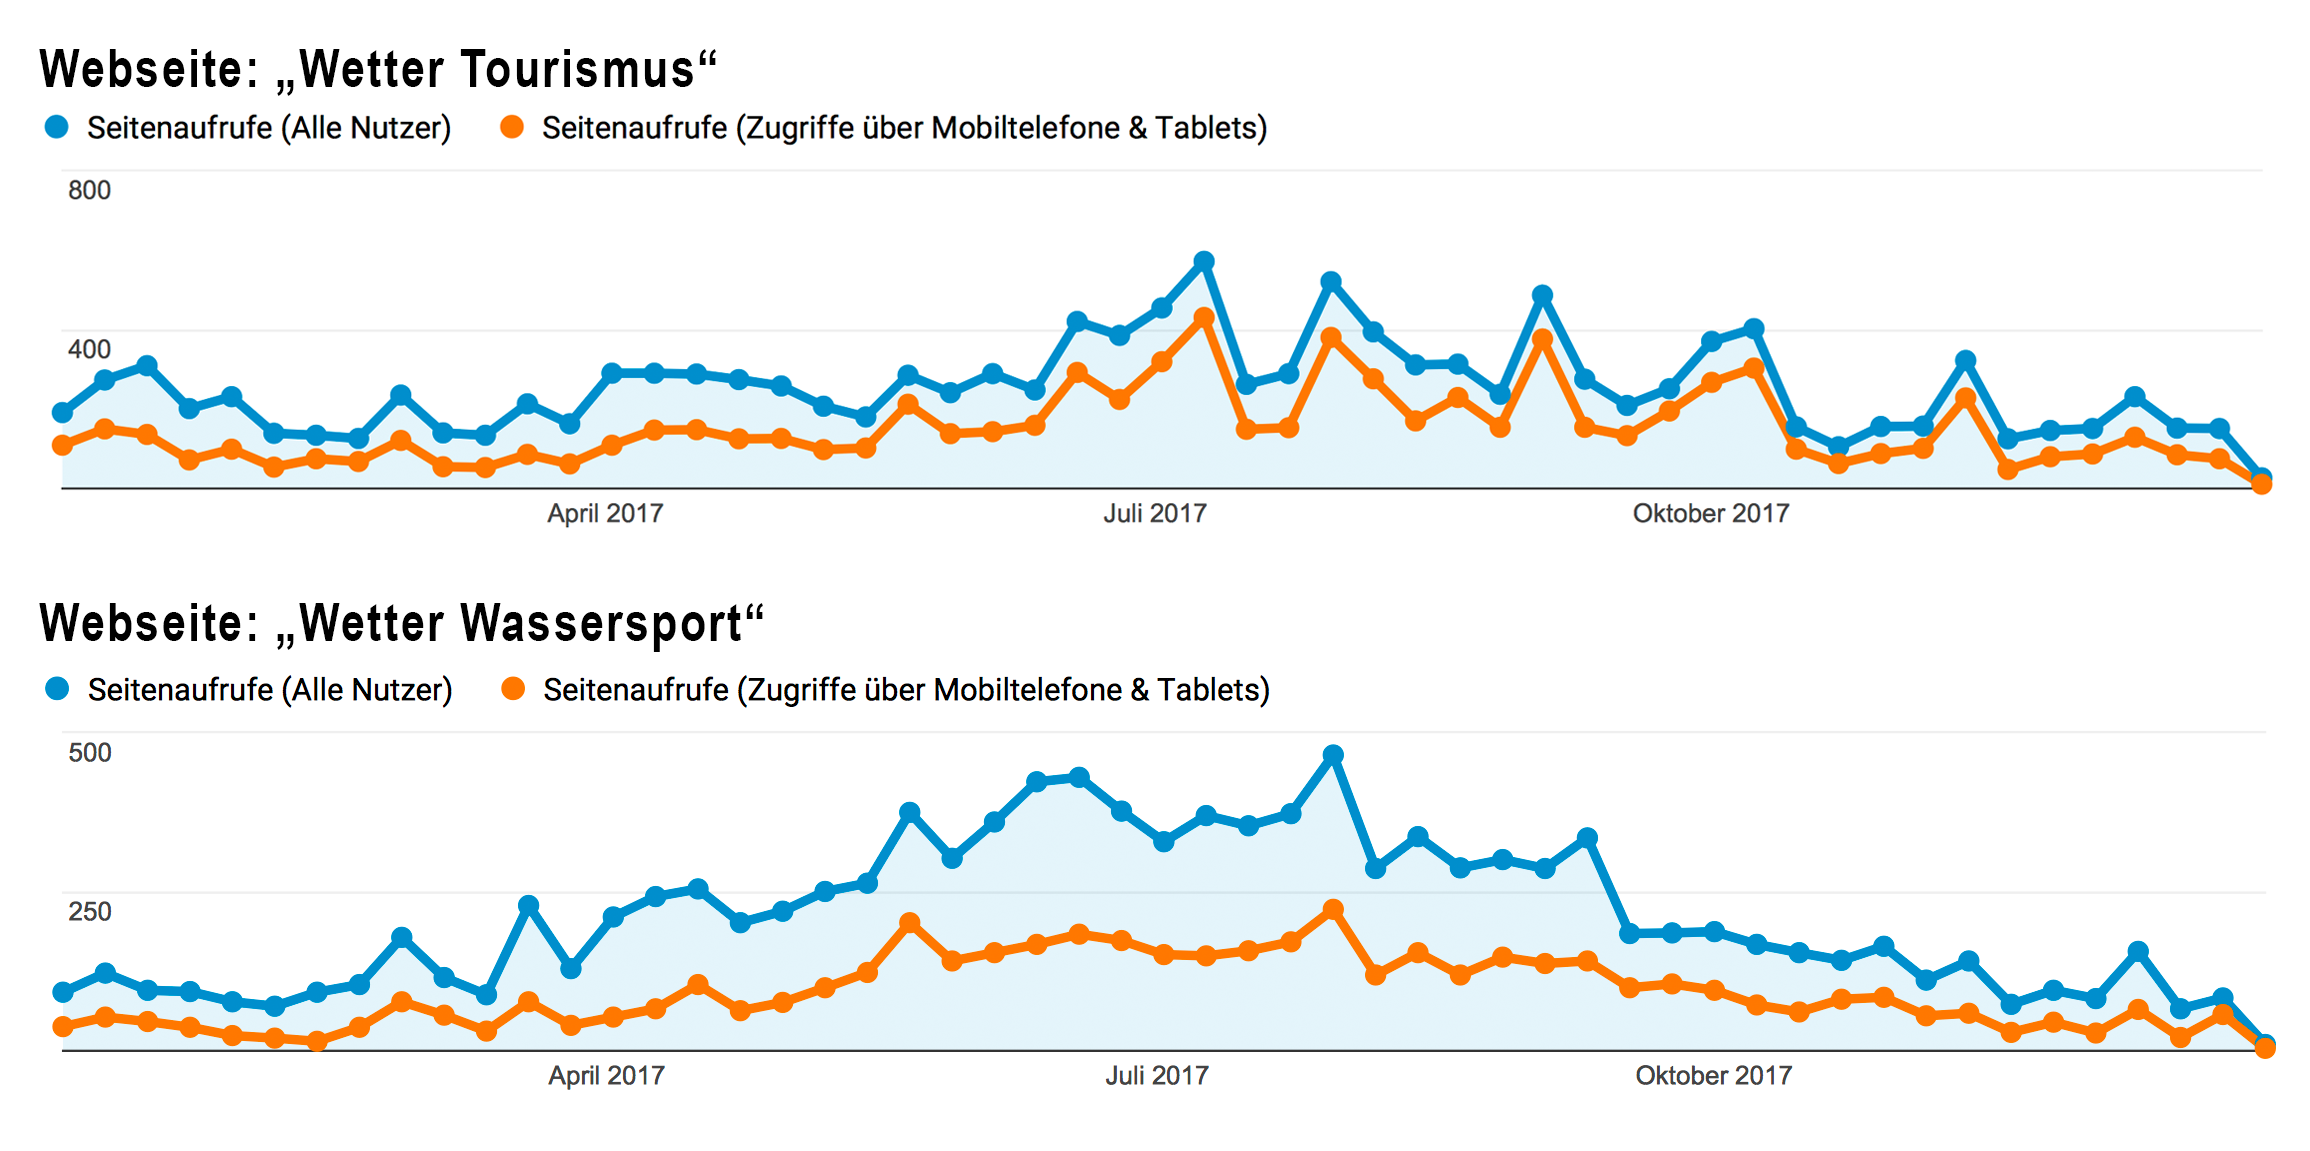
\includegraphics[width=\textwidth-2\fboxsep-2\fboxrule]{img/google_mobile}}
	\centering
	\caption{Anteil der mobilen Zugriffe auf die Wetterwebseite}
	\label{img:google_mobile}
\end{figure}

Es lässt sich ebenfalls erkennen welche Browser am häufigsten verwendet werden und welches die beliebteste Seite der Website ist, wie in Abbildung \ref{img:google_browser} dargestellt.

\begin{figure}[h!]
	\centering
	\fbox{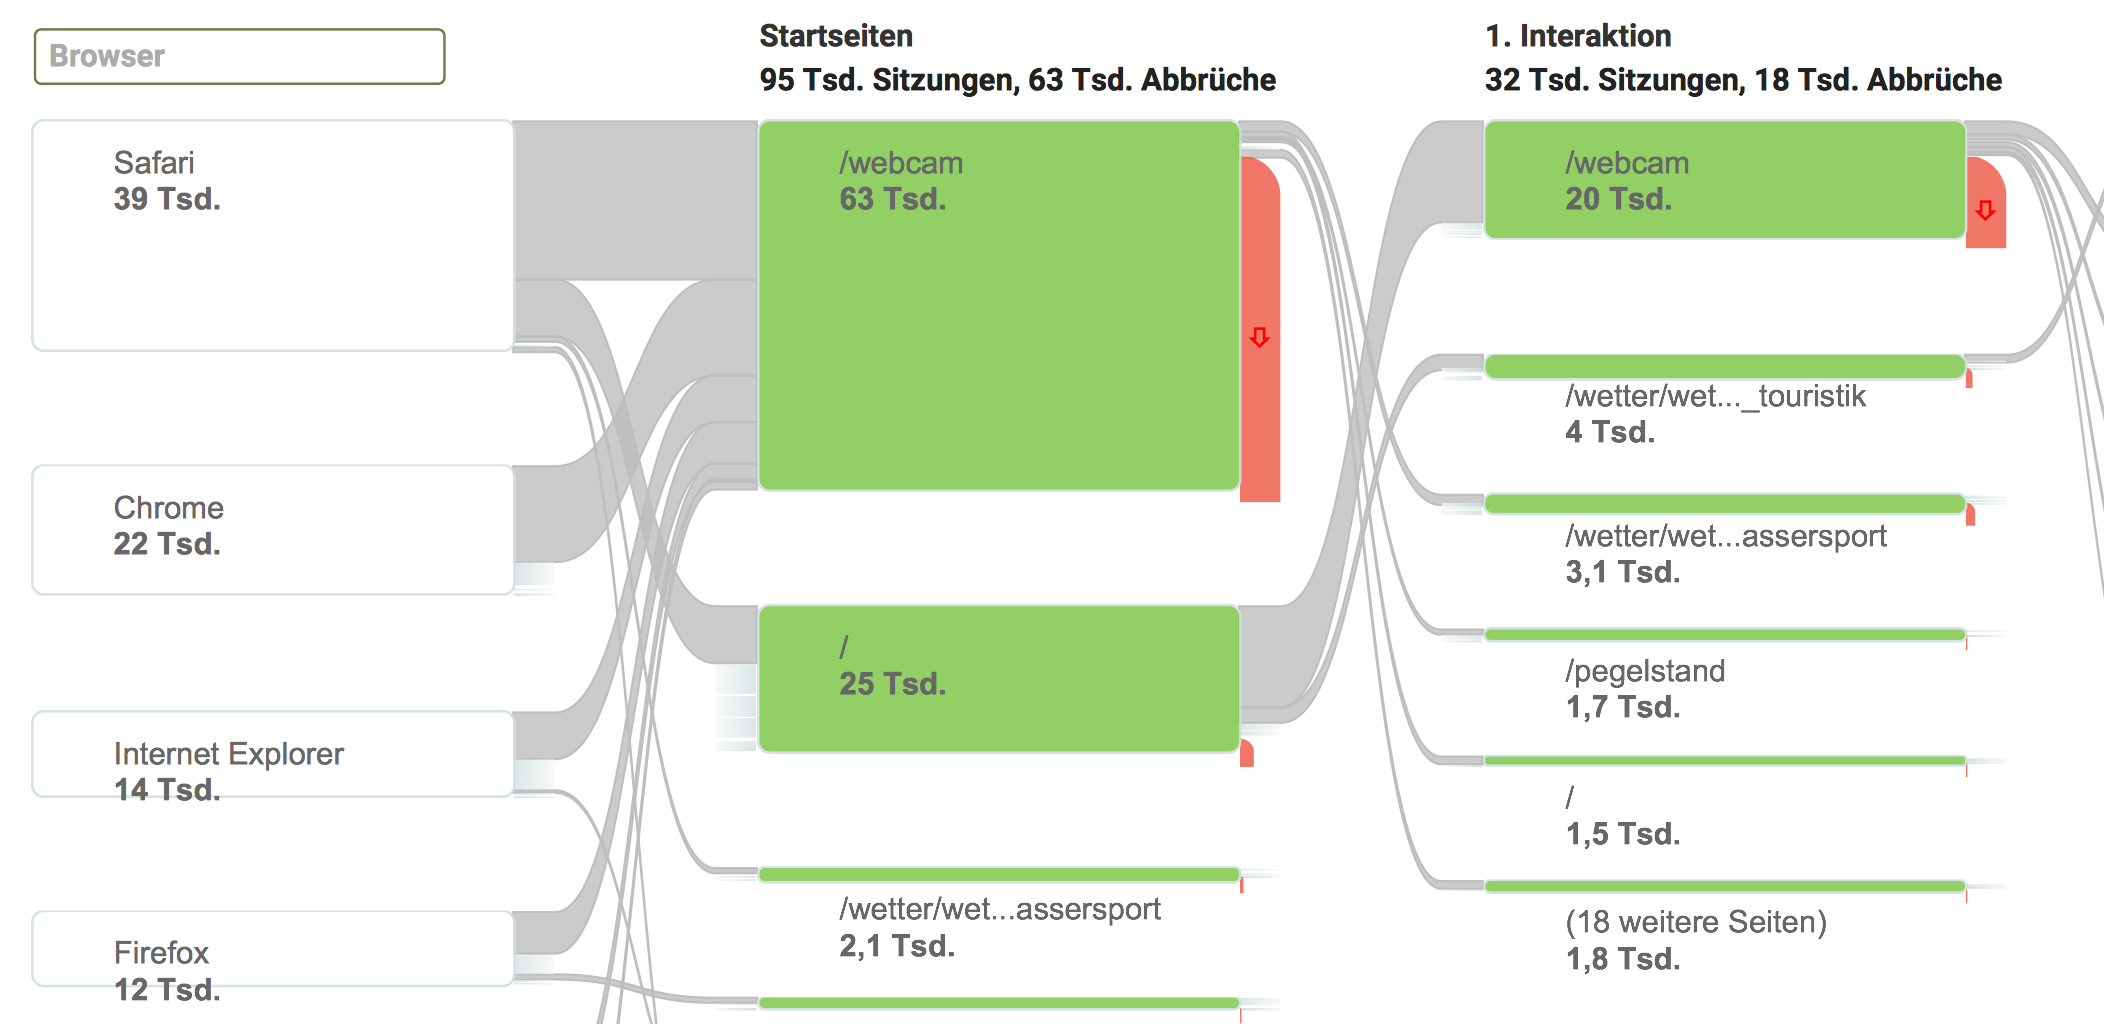
\includegraphics[width=\textwidth-2\fboxsep-2\fboxrule]{img/google_browser}}
	\caption{Verwendete Browser und Beliebtheit der Seiten}
	\label{img:google_browser}
\end{figure}



%% ############################################################################
%% Unterkapitel
%% ############################################################################
\subsection{Konzeption der crossplattformfähigen Benutzeroberfläche}
Wie im Abschnitt \ref{subsec:googleAnalytics} aufgezeigt werden bereits heute 50\% bis 80\% der Aufrufe von mobilen Geräten ausgeführt, Tendenz steigend. Es ist deshalb naheliegend das mobile Design als Startpunkt zu verwenden. Diese Vorgehensweise nennt sich \textit{Mobile First}. Es ist ein Designkonzept, das von Luke Wroblewski 2009 das erste Mal vorgeschlagen wurde. Die optimale Darstellung einer Website auf mobilen Endgeräten hat dabei oberste Priorität. Bei Mobile First beginnt der Designer mit dem Mobile-Design und arbeitet sich dann schrittweise zur grösseren Desktop-Version vor. Die \flqq Mobile Web Best Practices\frqq \footnote{ \url{https://www.w3.org/TR/mobile-bp}} des W3C empfiehlt zudem, dass sämtliche Informationen, die in der Desktop-Version zur Verfügung stehen, auch von der mobilen Seite aufgerufen werden können. Dieser Grundsatz nennt sich \textit{One Web Design}.

\begin{figure}[h!]
  \fbox{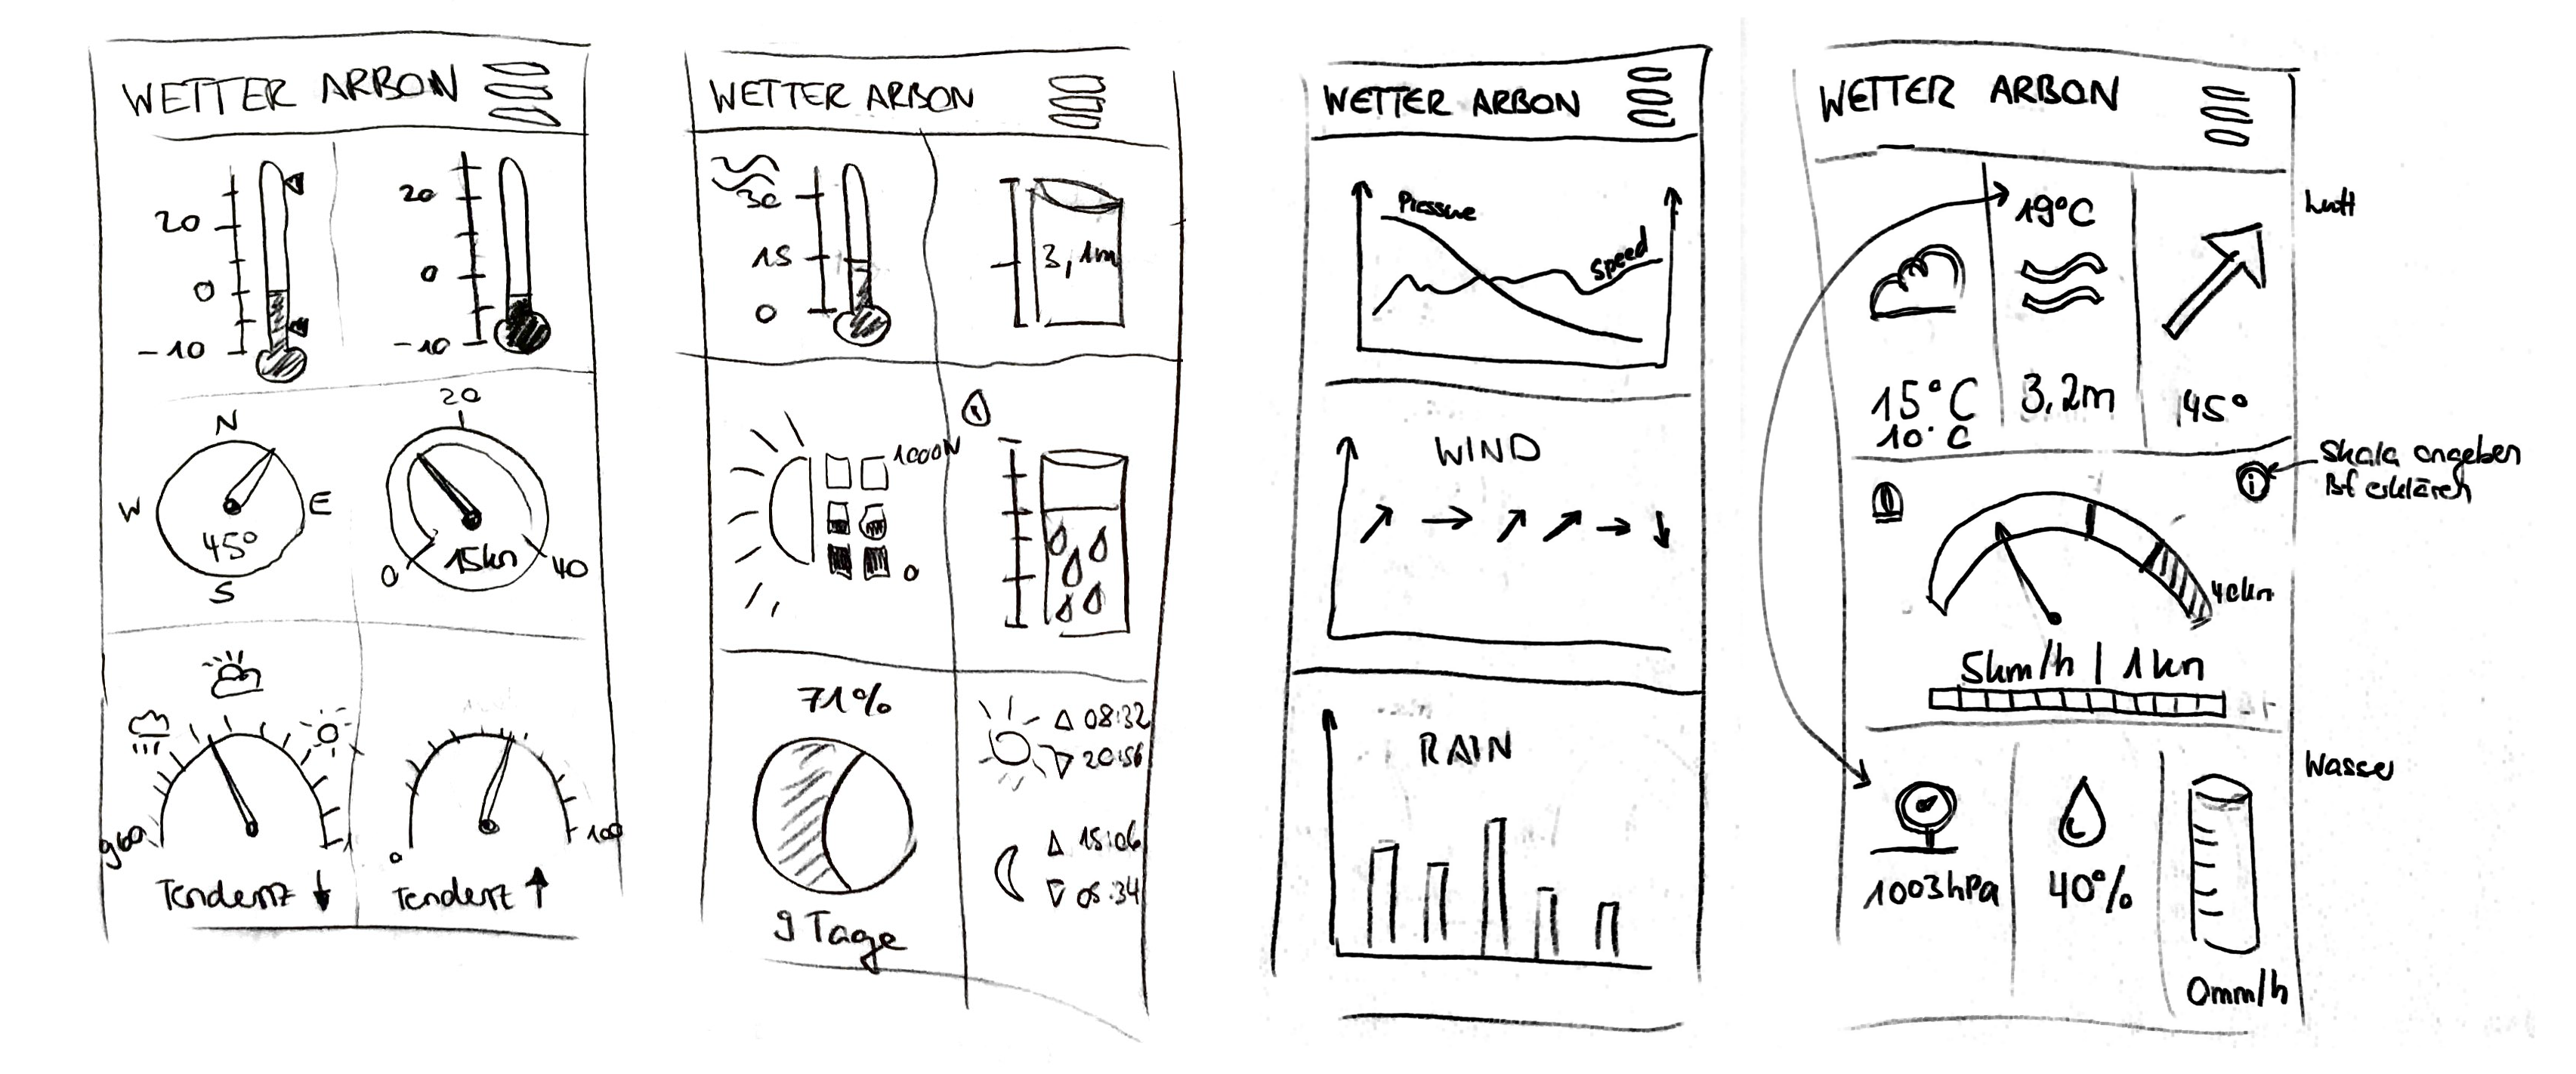
\includegraphics[width=\textwidth-2\fboxsep-2\fboxrule]{img/scribbles}}
	\centering
	\caption{Erste Designentwürfe nach dem Mobile First Prinzip}
	\label{img:scribbles}
\end{figure}

Beim Erstellen der ersten Designentwürfe, wie in Abbildung \ref{img:scribbles}, dargestellt, stellte sich schnell heraus, dass die einfachste Möglichkeit die Daten auf allen Bildschirmgrössen darzustellenzu können, darin besteht, die Informationen in kleine logische Blöcke zu unterteilen. Diese Blöcke können dann verschieden angeordnet werden. Dieses Kachel-Design ist eine gängiges Prinzip um das Gestaltungsgesetz der Zusammengehörigkeit umzusetzen und eignet sich hervorradend im Zusammenhang mit dem Grid-Konezpt des responsive Designs, welches im Abschnitt \ref{subsec:responsiveFactors} erläutert wird.


\subsubsection{W3.css als Layout-Framework}
Sämtliche Artefakte unserer Arbeit sollen möglichst einfach gehalten werden. Für die Gestaltung der Benutzeroberfläche haben wir uns deshalb entschlossen ein CSS-Framework zu benutzen. Dieses soll möglichst einfach und intuitiv zu bedienen sein, das Kachel-Design (auch Card-Design genannt) unterstützen, eine ausführliche Dokumentation aufweisen und eine geringe Dateigrösse haben. Wir haben drei verschieden CSS-Frameworks evaluiert und bewertet. Das Resultat ist in Tabelle  \ref{table:css-framework} ersichtlich.

\begin{table}[htb!]
\setlength\extrarowheight{3pt} % for a more "open" look
\begin{tabularx}{\textwidth}{|>{\RaggedRight\hspace{0pt}}p{4cm}||X|X|X|}

\hline
& \bfseries\large \href{https://www.w3schools.com/w3css/default.asp}{W3.css}
& \bfseries\large \href{https://purecss.io/start/}{Pure.css}
& \bfseries\large \href{http://getbootstrap.com/docs/4.1/getting-started/introduction/}{Bootstrap}\\

\hline
\textbf{Grid Design}
& ++
& ++
& ++ \\

\hline
\textbf{Footprint}
& 23 kB
& 14 kB
& 141 kB \\

\hline
\textbf{Usability}
& ++
& +
& + \\

\hline
\textbf{Card-Design}
& +
& -
& ++ \\

\hline
\textbf{Dokumentation}
& +++
& 0
& ++ \\

\hline
\textbf{Cross-Browser}
& ++
& ++
& +++ \\

\hline
\textbf{Funktionsumfang}
& +
& 0
& ++ \\

\hline
\end{tabularx}
\caption{Beurteilungsmatrix der evaluierten css-Frameworks}
\label{table:css-framework} % label muss NACH caption stehen!!!!
\end{table}

\noindent
Als Sieger stellt sich das W3.css-Framework heraus, da es den besten Kompromiss zwischen Dateigrösse und Funktionsumfang bietet. Zumdem weist es eine hervorragende Dokumentation auf.


\subsubsection{Responsive Design}
\label{subsec:responsiveFactors}
Die Benutzeroberfläche muss Cross-Plattform-fähig sein d.h. die Darstellung muss sich je nach Bildschirmgrösse automatisch anpassen. Man nennt dies \textit{Responsive Design}. Die Idee des Responsive Web Design wurde 2010 von Ethan Marcotte in einem Artikel\footnote{ \url{http://alistapart.com/article/responsive-web-design}} des Magazins \textit{A List Apart} veröffentlicht. Hintergrund war, dass man nicht für jedes neue Gerät eine eigene Webseite erstellen wollte. Marcotte schreibt von drei Faktoren, die ein responsive Design benötigt: Fluid grids, flexible images und media queries. Fluid grids bedeutet, dass sich die Anordnung der Elemente dynamisch der Bildschirmgrösse anpasst. Flexible Bilder haben keine feste Grösse sondern nutzen den ihnen zu Verfügung stehenden Platz optimal aus und die Media queries sind die technische Basis für die beiden oberen Anforderungen.

\begin{figure}[h!]
  \fbox{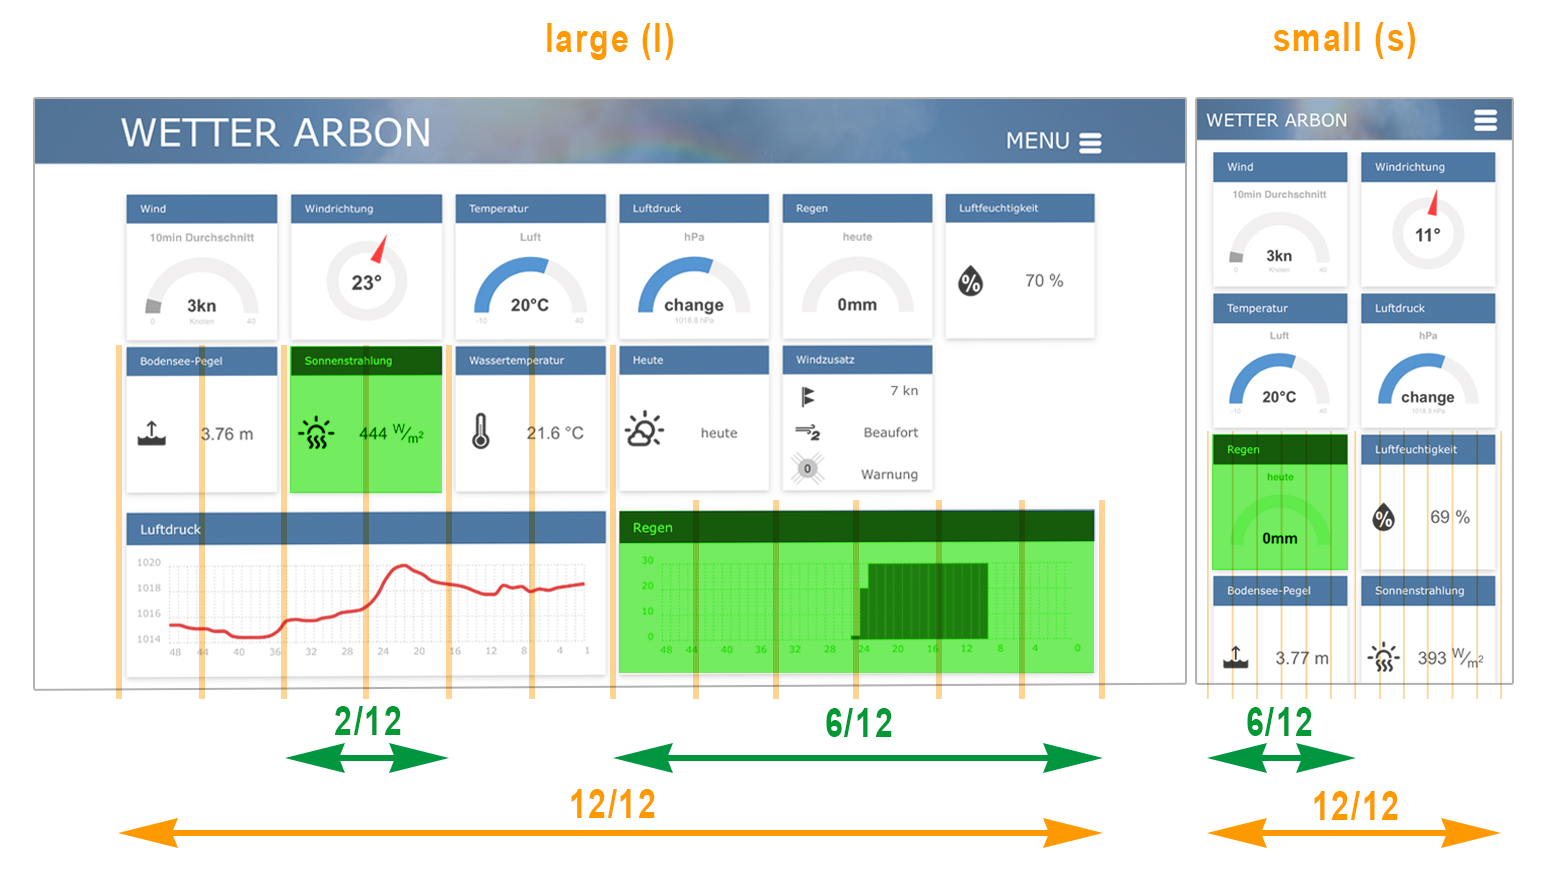
\includegraphics[width=\textwidth-2\fboxsep-2\fboxrule]{img/kacheln2}}
	\centering
	\caption{Anordnung der Kacheln auf grossen und kleinen Bildschirmen}
	\label{img:kacheln2}
\end{figure}

\noindent
Das Konezt des Grid-View teilt den Bildschirm in zwölf Spalten ein. Über eine media-Query fragt die Webseite die Grösse des Bildschirms ab. Es gibt drei Kategorien small, medium, large, deren Grenzen folgendermassen festgelegt sind:

\begin{itemize}
\item Small: s $\leq$ 600px (z.B. iPhone Hochformat)
\item Medium: 600px < m $\leq$ 992px (z.B. iPhopne Querformat, iPad Hochformat)
\item Large: 993px < l (z.B. Desktop)
\end{itemize}

\noindent
Im css-Framework kann nun sehr einfach definiert werden wie sich die Kacheln bei diesen drei Bildschirmkategorien verhalten sollen. Die Kacheln der aktuellen Daten sind auf grossen (large) Bildschirmen \nicefrac{2}{12}, auf mittleren Bildschirmen \nicefrac{3}{12} und auf kleinen Bildschirmen \nicefrac{6}{12} breit. Bei den Datenverläufen werden bei mittleren und grossen Bildschirmen zwei nebeneinander dargestellt, bei kleinen Bildschirmen alle untereinander.

\begin{lstlisting}[label=lst:kacheln,caption=Konfiguration der Anzahl Kacheln abhähngig von der Bildschirmgrösse, language=HTML5, style=htmlcssjs]
<!-- Aktuelle Daten -->
<div class="w3-col l2 m3 s6">
	<div class="w3-card">...</div>
</div>

<!-- Datenverlauf -->
<div class="l6 m6 s12">
	<div class="w3-card">...</div>
</div>
\end{lstlisting}

%% ############################################################################
%% Unterkapitel
%% ############################################################################
\subsection{Grafische Darstellung der aktuellen Wetterdaten}
Die Anzeigeelemente für die aktuellen Messwerte sollen ebenfalls mit Hilfe eines Frameworks erstellt werden. Damit die Grafiken optimal mit dem responsive Layout zusammenspielen, müssen sie ein flexibles Layout aufweisen d.h. ihre Grösse dem vorhanden Platz anpassen. Am Besten nicht nur beim Aufrufen der Seite, sondern auch beim Ändern der Fenstergrösse. Zudem muss es einfach möglich sein die Werte zu aktualisieren.

Die Anzeige sollte möglichst ein klares Design aufweisen aber trotzdem individuell anpassbar sein. Ein sehr einfaches JavaScript-Framework ist \textit{JustGage}\footnote{ \url{http://justgage.com}}. Die Grafiken lassen sich über eine JavaScript-Datei konfigurieren, die Grafiken selbst sind im svg-Format und somit von praktisch allen Browsern darstellbar. JustGage basiert auf der \textit{Raphaël}\footnote{ \url{http://dmitrybaranovskiy.github.io/raphael/}}—JavaScript Bibliothek.

\begin{figure}[h!]
  \fbox{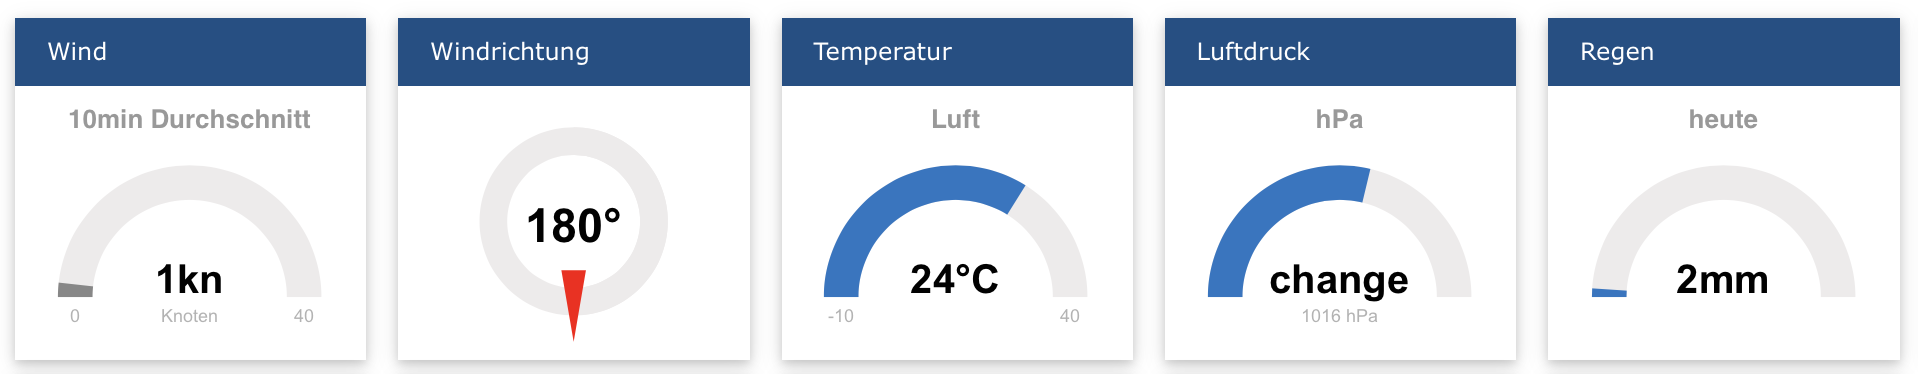
\includegraphics[width=\textwidth-2\fboxsep-2\fboxrule]{img/gauges}}
	\centering
	\caption{Anzeigelemente mit Justgage/Raphaël}
	\label{img:gauges}
\end{figure}

Raphaël ist eine kleine JavaScript-Bibliothek, die Ihnen die Arbeit mit Vektorgrafiken im Web erleichtern soll. Wenn Sie z.B. Ihr eigenes Diagramm oder Bildausschnitt erstellen und das Widget drehen möchten, können Sie dies einfach und bequem mit dieser Bibliothek erreichen. Raphaël verwendet die SVG W3C Recommendation und VML als Grundlage für die Erstellung von Grafiken. Dies bedeutet, dass jedes grafische Objekt, das Sie erstellen, auch ein DOM-Objekt ist, so dass Sie JavaScript-Ereignisbehandler anhängen oder später ändern können. Raphaëls Ziel ist es, einen Adapter zur Verfügung zu stellen, der das Zeichnen von Vektorgrafiken browserübergreifend und einfach macht.


\begin{lstlisting}[label=lst:gaugeJS,caption=Konfiguration der Gauge, language=JavaScript,mathescape, style=htmlcssjs]
var temperature_gauge = new JustGage({
  id:     temperature_gauge,
  value:  initialValues.v1.data.temperature.value,
  min:    -10,
  max:    40,
  symbol: C,
  title:  Luft
});
\end{lstlisting}

Um die Grafik anzuzeigen muss nur ein DIV mit der selben ID auf der Webseite erstellt werden wie in Listing \ref{lst:gaugeHTML} dargestellt.

\begin{lstlisting}[label=lst:gaugeHTML,caption=Container für die SVG-Grafik (Gauge), language=HTML5, style=htmlcssjs]
<!-- Lufttemperatur -->
<div class="w3-cell w3-col l2 m3 s6">
  <div class="w3-card">
    <div class="w3-container">
      <p>Temperatur</p>
    </div>
    <div id="temperature_gauge" class="gauge"></div>
  </div>
</div>
\end{lstlisting}

Die Messwerte sind einerseits über den Titel beschrieben, sie enthalten aber zusätzlich ein passendes Icons. Es wurde eine Icon-Bibliothek gewählt, die möglichst alle benötigen Icons enthält, die kostenlos ist, und deren Grafiken im svg-Format vorliegen. Als geeignet schienen die \textit{Weahter Icons}\footnote{\url{http://erikflowers.github.io/weather-icons/}} von Erik Flowers.


\begin{figure}[h!]
  \fbox{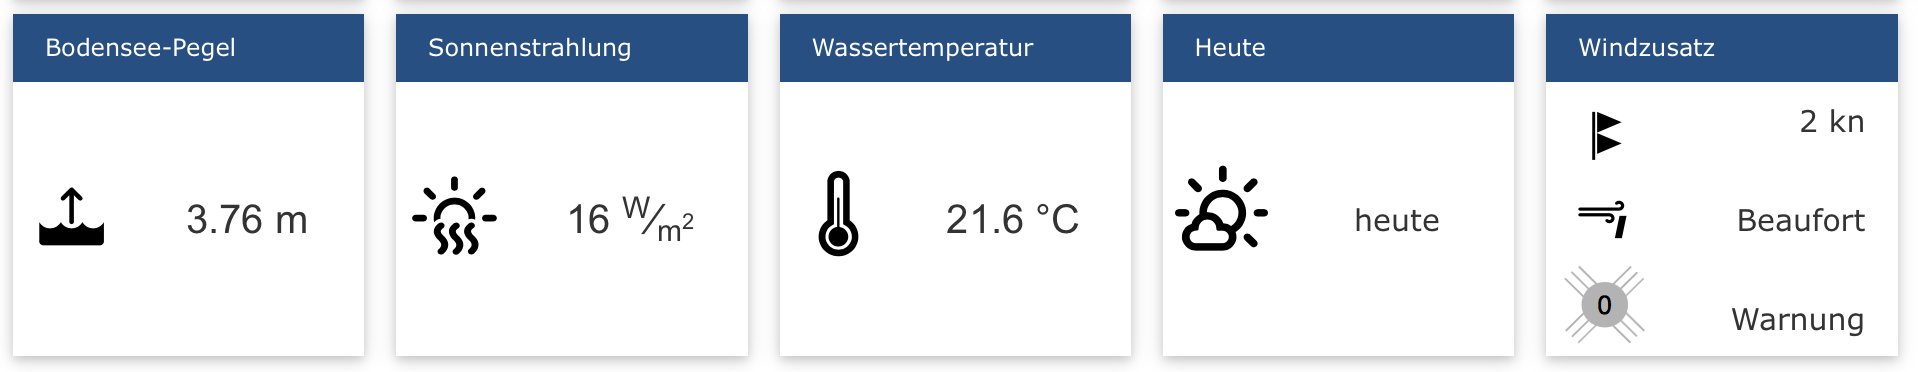
\includegraphics[width=\textwidth-2\fboxsep-2\fboxrule]{img/icons}}
	\centering
	\caption{Icons aus der Weather Icons Bibliothek}
	\label{img:icons}
\end{figure}





%% ############################################################################
%% Unterkapitel
%% ############################################################################
\subsection{Grafische Darstellung der Wetterdatenverläufe}
Die Wetterverlaufsdarstellung soll einen Überblick über die Wettertendenz der letzten beiden Tage liefern. Die Samplerate beträgt 1h, d.h. die Daten werden aus der Tabelle der historischen Werte abgerufen.

\begin{figure}[h!]
  \fbox{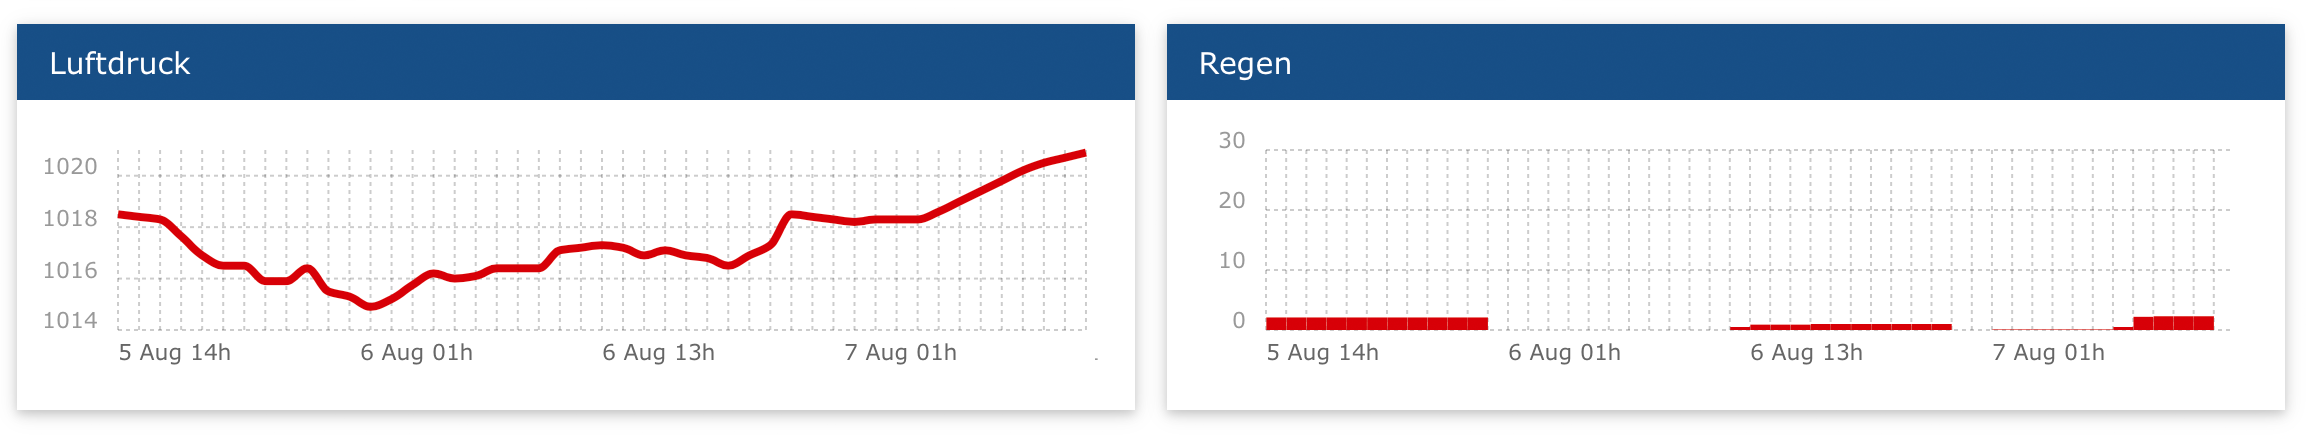
\includegraphics[width=\textwidth-2\fboxsep-2\fboxrule]{img/charts}}
	\centering
	\caption{Verlaufsdiagramm mit chartist.js}
	\label{img:charts}
\end{figure}



\subsubsection{Auswahl des JS-Frameworks}
Für die Darstellung der Messwertverläufe soll ebenfalls auf eine Bibliothek zurückgegriffen werden. Als erstes wurden js-Bibliotheken gesucht, die ein ansprechendes Design aufweisen. Übrig geblieben sind die in Tabelle \ref{table:js-framework} aufgeführten drei js-Bibliotheken. Diese wurden auf ihre Eignung geprüft. Zwingend mussten die Grafiken im SVG-Dateiformat vorliegen, sodass die Cross-Browser-Kompatiblität und das responsive Verhalten sichergestellt ist. Die Daten sollten zudem als JSON übergeben werden können. D3 ist zwar DIE js-Bibliothek wenn es um Visualisierungen im Web geht, hat aber keine vorgefertigten Diagramme und benötigt entsprechend viel Aufwand und Einarbeitungszeit, was wir explizit nicht möchten.

\begin{table}[htb!]
\setlength\extrarowheight{3pt} % for a more "open" look
\begin{tabularx}{\textwidth}{|>{\RaggedRight\hspace{0pt}}p{3.5cm}||X|X|X|}

\hline
& \bfseries\large \href{https://gionkunz.github.io/chartist-js/index.html}{chartist.js}
& \bfseries\large \href{https://www.fusioncharts.com}{Fusion Charts}
& \bfseries\large \href{https://developers.google.com/chart/}{Google Charts}\\

\hline
\textbf{Footprint}
& 10 kB
& >1000 kB
& 110 kB \\

\hline
\textbf{Barrierefrei}
& +
& 0
& + \\

\hline
\textbf{Anpassbarkeit}
& ++
& +++
& ++ \\

\hline
\textbf{Dokumentation}
& +++
& +++
& ++ \\

\hline
\textbf{Kostenlos}
& +
& --
& + \\

\hline
\textbf{Funktionsumfang}
& ++
& +++
& + \\

\hline
\end{tabularx}
\caption{Beurteilungsmatrix der evaluierten js-Frameworks}
\label{table:js-framework} % label muss NACH caption stehen!!!!
\end{table}

\noindent
Chartist.js stellte den besten Kompromiss zwischen Funktionsumfang, Einfachheit und Dokumentation dar. Insbesondere die Dateigrösse war ausschlaggebend, da die Webseite, wie in Abschnitt \ref{subsec:googleAnalytics} erklärt, primär von mobilen Nutzer genutz wird.

% Code-Beispiel
\begin{lstlisting}[label=lst:charts,caption=Konfiguration der Verlaufsdiagramme, language=HTML5, style=htmlcssjs]
//Luftdruck
var Barometer = {
  labels: [48,...,1],
  series: [dataBarometerHistoric]
};
new Chartist.Line('#air-chart', Barometer);

//Regen
var Rain = {
	labels: [48,...,1],
	series: [dataRainHistoric]
};
var options = {
low: 0,
high: 30,
};
new Chartist.Bar('#rain-chart', Rain, options);
\end{lstlisting}
\ \\


Zur Verlaufsdarstellung wird primär das Linien- und Balkendiagramm verwendet, wie in Abbildung \ref{img:charts} aufgezeigt. Für jede Grafik wurde entschieden ob eine automatische Y-Achs-Skalierung sinnvoll ist oder nicht. Bei der Windgeschwindigkeit und beim Pegel wurd bewusst eine fixe Skalierung verwendet, damit auf den ersten Blick klar ist, ob der Wert eher hoch oder eher tief ist. Beim Luftdruck hingegen ist die Tendenz wichtig, weshalb möchglichst die gesamte Höhe des Diagramms genutzer werden soll. Es wird daher eine automaitsche Y-Achs-Skalierung verwendet. Die Konfiguration erfolgt in einem einfach JS-File wie in Listing Listing \ref{lst:charts}  dargestellt. Unter \textit{options} kann die y-Achse auf die gewünschten Werte fixiert werden.\newline


\subsubsection{Anzeige der Windrichtung}
Die Anzeige des Windrichtungsverlaufs ist nicht ganz trivial da sie von 0 bis 360 Grad geht und ohne Unterbruch wieder zu 0 Grad. In der Praxis wird dazu häufig die Darstellung von Pfeilen verwendet wie in Abbildung \ref{img:windrichtung}, links dargestellt. Es konnt jedoch kein Framework gefunden werden, das diese Darstellungsart als Template zur Verfügung stellt. Die Anzeige der Windrichtung wird deshalb über ein Punktdiagramm, wie in Abbildung \ref{img:windrichtung}, rechts dargestellt verwendet.

\begin{figure}[h!]
	\centering
  \fbox{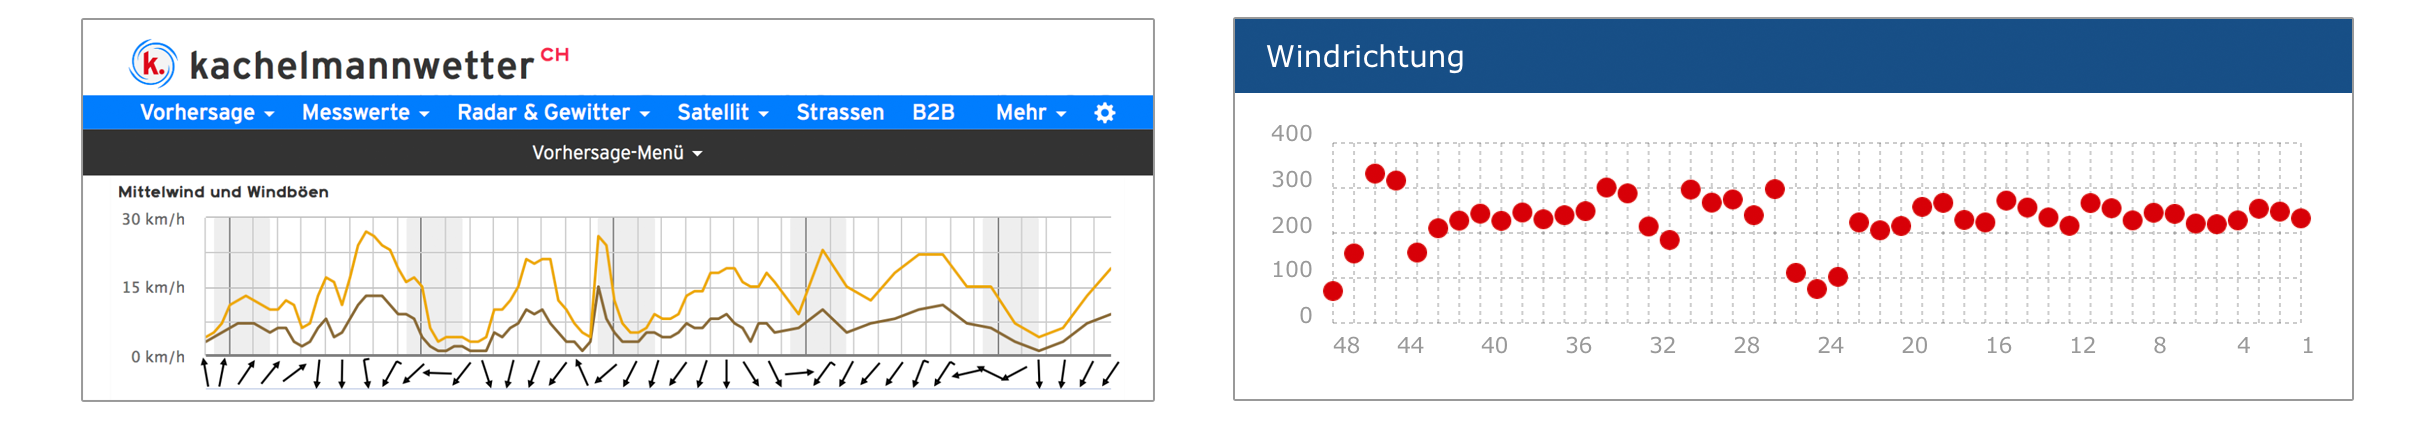
\includegraphics[width=\textwidth-2\fboxsep-2\fboxrule]{img/windrichtung}}
	\caption{Windrichtungsanzeige soll und ist}
	\label{img:windrichtung}
\end{figure}

\subsubsection{Vergleich Prognose/Ist Windgeschwindigkeit}
Insbesondere bei Seglern sind Windprognosenseiten sehr beliebt. Sie liefern Windprognosen bis zu fünf Tage voraus. Bei allen Vorhersagediensten ist nicht erkennbar wie gut dir Prognose war. Geanu dies ist aber eine spannende Frage weshalb dieser Vergleich auf der Webseite angezeigt werden soll. Die Messdaten der Wetterstation werden daher mit zwei kostenlosen Vorhersagediensten verglichen. Dabei wird jeweils die Dreitagesvorschau betrachtet. Für die Windvorhersage wurden folgende zwei Anbieter ausgewählt:

\begin{itemize}
\item Openweathermap
\item Windfinder
\end{itemize}

\noindent
Opeanwathermap ist einer der wenigen Anbieter, der eine kostenlose API zur Verfügung stellt. Windfinder ist unter den Seglern das beliebteste Tool. Die Vorhersagedaten werden von den Anbietern nur in die Zukunft angezeigt d.h. wie die Vorhersage von gestern war ist nicht mehr ersichtlich. Aus diesem Grund müssen die Vorhersagedaten abgegriffen und gespeichert werden. Für den Prognoseanbieter haben wir uns für Openweathermap und windfinder entschieden. OWM bietet eine kostenlose Web-API. Windfinder ist eines der beliebtesten Seglertools, bietet aber keine API sondern lediglich ein Widget für den gewünschten Standort an. Dies Daten müssen somit aus dem Windfinder-Widget, siehe Abbildung \ref{img:windfinder}, mittels Crawler extrahiert werden, analog Listing \ref{lst:kttgCrawler}.

\begin{figure}[h!]
	\centering
  \fbox{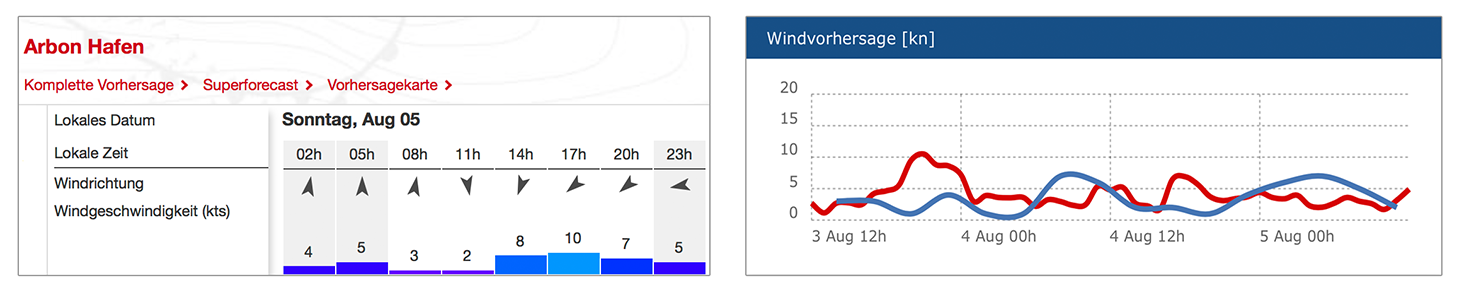
\includegraphics[width=\textwidth-2\fboxsep-2\fboxrule]{img/windfinder}}
	\caption{Widget von Windfinder}
	\label{img:windfinder}
\end{figure}

Nach den ersten Auswertungen wurde festgestellt, dass die Wettervorhersagedaten von Openweathermap absolut unbrauchbar waren. Sie lagen permanent zwischen 0 und 1 Knoten auch wenn die Wetterstation 15 Knoten messte. Die Vorhersage von Openweathermap wurde deshalb nicht mehr weitervervolgt.

Die Abfrage der Datenban stellt sich als recht kompliziert heraus. Sodass entschieden wurde eine VIEW einzusetzten. Diese wird dynamisch bei Aufrufen erzeugt und enthält die gewünschten Daten. Der SQL-Befehl für die Erzeugung der VIEW ist vereinfacht in Listing \ref{lst:viewForecast} aufgeführt. Primär gibt es zwei Bediungungen. Erstens sollen nur die Dreitageverhersagewerte verwendet werden und zweitens sollen die Vorhersagewerte verwendet werden, die am nächsten bei der aktuellen Zeit liegen. Da das Vorhersageintervall 3 Stunden beträgt ist die Verhersage maximal 1.5 Stunden verschoben.

%View erstellen
\begin{lstlisting}[label=lst:viewForecast,caption=Erzeugung der VIEW für den Forecast-Vergleich, language=SQL, style=htmlcssjs]
SELECT *
FROM 'tblcompwindfinder'
WHERE
(datetime + interval 3 day) <= now() #heute vor drei Tagen
AND
abs(timediff(datetime,now())) <= 13000) #innerhalb +/- 1.5h
ORDER BY datetime DESC
LIMIT 3
\end{lstlisting}

%\Diskussionspunkt{- Eintagesvorschau}\newline
%\Diskussionspunkt{- Mittels Tableau? Eigen Webseite?}\newline
%\Diskussionspunkt{- Bild mit Vergleich von Messwerten, Vorhersage Windfinder und Vorhersage Openweathermap}\newline

% Graphen, der den heutigen Tag, links davon die letzten 14 Tage und rechts davon die nächsten drei Tage anzeigt.
% Pro Anbieter und Prognoseart (1Tag bzw. 3 Tage) wird ein eigener Graph erstellt.
% Aus diesen Gründen wird die Webseite zwar veröffentlicht, aber kein Link dazu auf der Webseite zur Verfügung gestellt.
% Werte aus der Stundenwert-Datenbank?

%% ############################################################################
%% Unterkapitel
%% ############################################################################
\subsection{Anzeige der aktuellen Sturmwarn-Situation}
\label{subsec:sturmwarnung}

% was ist der Sturmwarndienst und wie werden die verschiedenen Stufen dargestellt
Auf dem Bodensee gibt es einen Sturmwarndienst, der die Schiffsführer vor aufkommendem Sturm warnen soll. Der Sturmwarndienst wird vom Deutschen Wetterdienst in Zusammenarbeit mit MeteoSchweiz betrieben. Rund um den Bodensee sind dafür über 60 Sturmwarnleuchten installiert (Abbildung \ref{img:sturm2}). Es wird unterschieden zwischen \textit{Starkwindwarnung} und \textit{Sturmwarnung}. Erstere weist auf auf starke Windböen zwischen 25 Knoten und 33 Knoten hin und wird durch Aufleuchten von orangefarbigen Blinklichtern mit ca. 40 orangefarbigen Blitzen pro Minute an den Sturmwarnleuchten signalisiert. Letzere kündigt das Auftreten von Windböen von 34 Knoten und mehr an und wird durch Aufleuchten von orangefarbigen Blinklichtern mit ca. 90 orangefarbigen Blitzen pro Minute an den Sturmwarnleuchten signalisiert (gemäss Anlage B der Bodensee-Schifffahrts-Ordnung\footnote{ \url{https://www.admin.ch/opc/de/classified-compilation/19760005/index.html}}, BSO).

\begin{figure}[h!]
	\centering
  \fbox{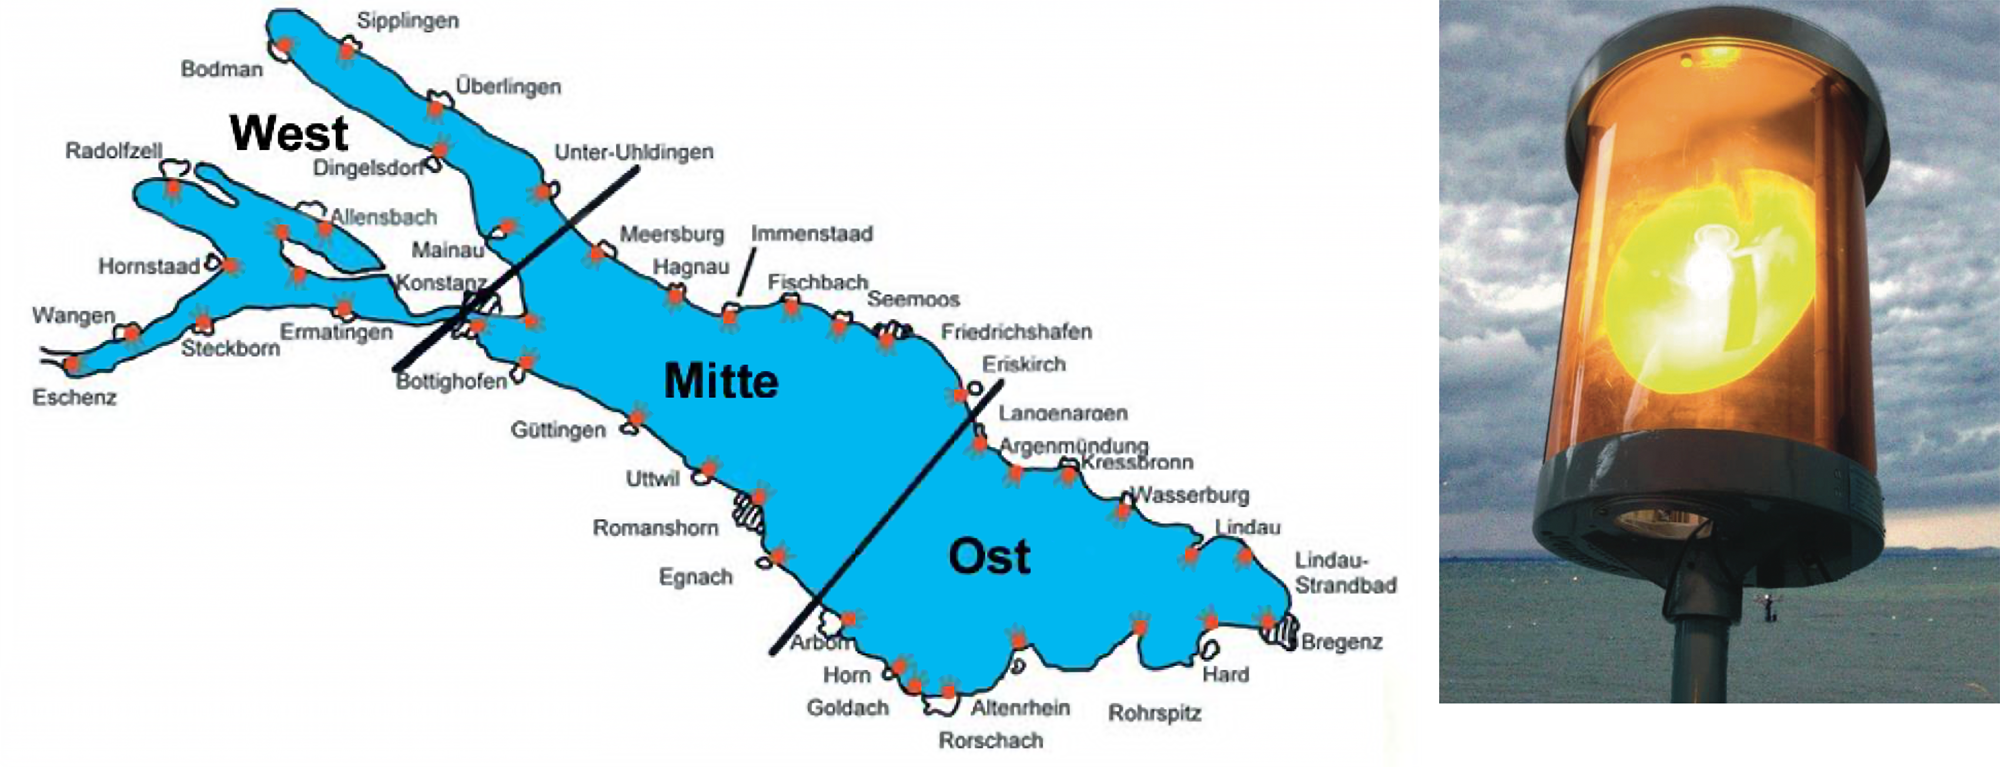
\includegraphics[width=\textwidth-2\fboxsep-2\fboxrule]{img/sturm2}}
	%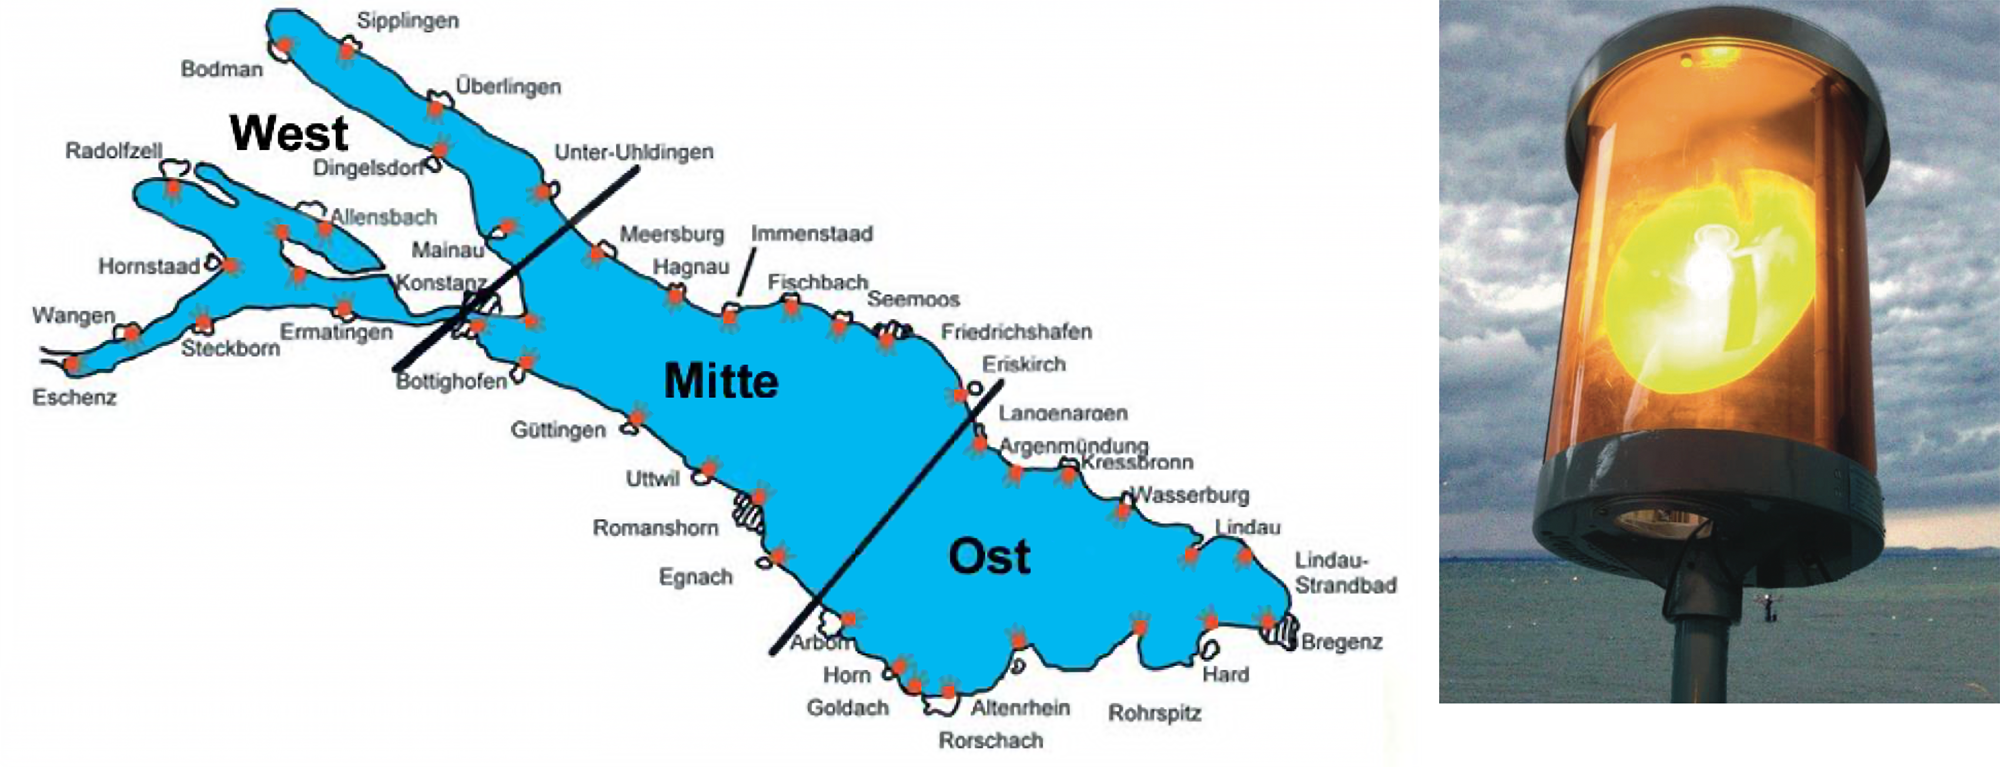
\includegraphics[width=1\linewidth]{img/sturm2}
	\caption{Sturmwarndienst Bodensee}
	\label{img:sturm2}
\end{figure}

% Problem: Kostenpflichtige Informaiton
Den aktuellen Status der Sturmwarnung kann sowohl beim Deutschen Wetterdienst, als auch bei meteoschweiz kostenpflichtig bezogen werden (ca. 1300CHF/Jahr). Kostenlos gibt es nur zwei browserkomatible Quellen: Das eine ist die allgemeine Mini-Warnkarte (173 x 109 Pixel) von meteoschweiz (siehe Abbildung \ref{img:sturm}, links) und das andere ist die Anzeige auf der Webseite der Kantonspolizei, Abbildung \ref{img:sturm}, rechts.

\begin{figure}[h!]
	\centering
  \fbox{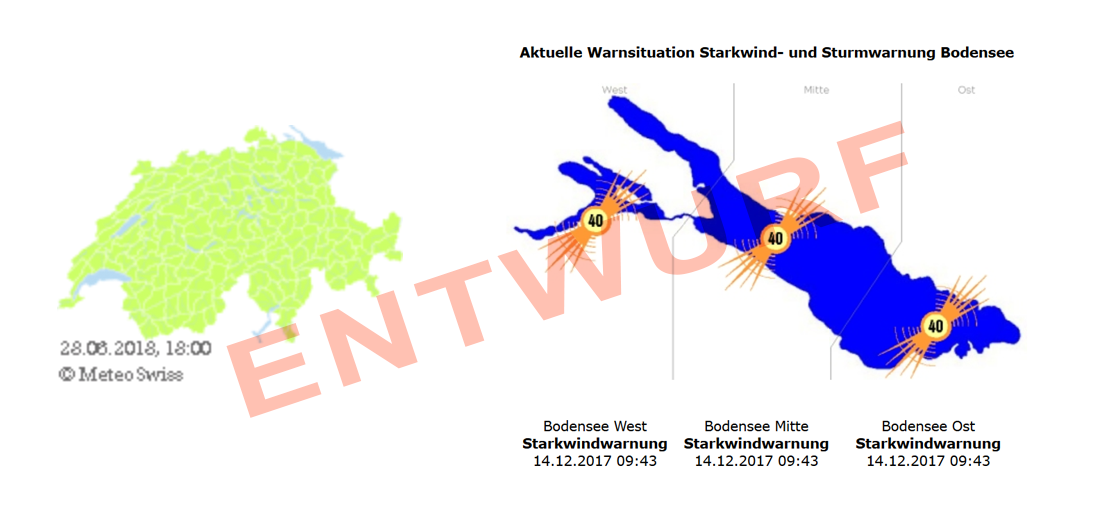
\includegraphics[width=\textwidth-2\fboxsep-2\fboxrule]{img/sturm}}
	%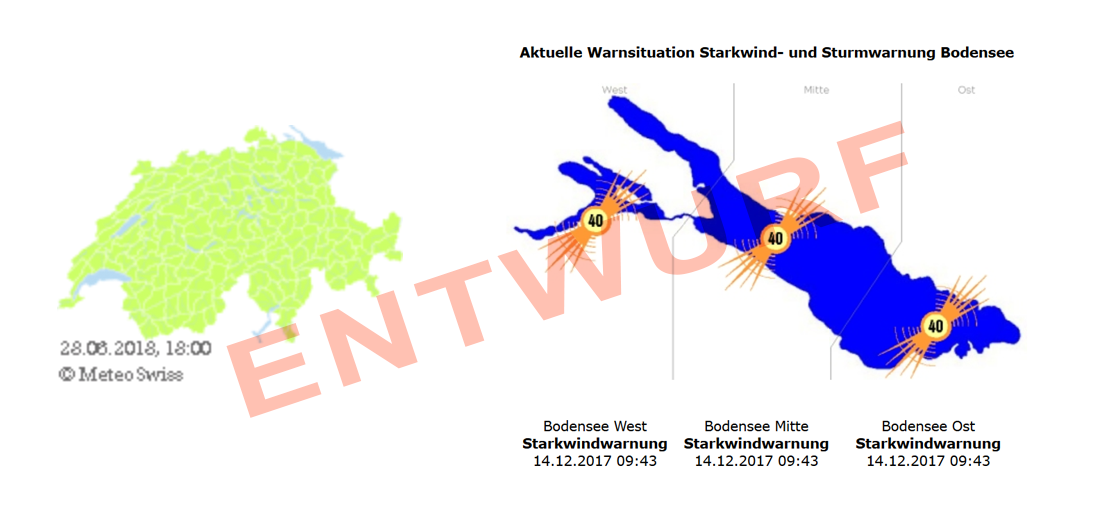
\includegraphics[width=1\linewidth]{img/sturm}
	\caption{Kostenlose Browserdarstellung}
	\label{img:sturm}
\end{figure}

Eine kostenlose API steht nicht zur Verfügung. Meteoschweiz verbietet es, Informaitonen von ihrer Website abzugreifen. Wir haben deshalb beim Amt für Informatik des Kantons Thurgau die Erlaubnis eingeholt, die Sturmwarndaten von der Kapo-Webseite abgreifen zu dürfen. Wir verwenden dazu die Python Bibliothek \textit{BeautifulSoup} als web crawler, wie in Listing \ref{lst:kttgCrawler} dargestellt. \newline

\begin{lstlisting}[label=lst:kttgCrawler,caption=Web Crawler für die Sturmwarndaten, language=python, style=py]
page = requests.get('http://www.kttg.ch/kapo/htm/stwarn.shtml')
soup = BeautifulSoup(page.text, 'html.parser')

# Einschaltzeit auslesen
soup.select('table tr:nth-of-type(4) td'):

# Status auslesen
soup.select('.titelfett strong'):
\end{lstlisting}

% Problem 1: keine API -> wenn Seite ändert, muss Crawler angepasst werden.
Das Problem beim Verwenden des Web Crawlers besteht darin, dass sobald die URL oder die Webseite geändert wird, der Crawler angepasst werden muss. Da der Crawler jedoch die einzige kostenlose Möglichkeit darstellt um die Daten zu erhalten, müssen wir dieses Risiko akzeptieren.

% Problem 2: Öffnungszeiten -> keine Warnung in der NAcht
Der Sturmwarndienst wie in Abschnitt \ref{subsec:sturmwarnung} beschrieben, ist kein 24h-Service. Der Dienst ist nur tagsüber aktiv zu den aufgelisteten Warnzeiten\footnote{ \url{https://kapo.tg.ch/public/upload/assets/56408/A5\%20Sturmwarnung.pdf}}, was aus Sicht der Sicherheit auf dem See nicht sehr sinnvoll ist.

\begin{itemize}
\item 1. April - 31. Oktober: 06:00 - 22:00 Uhr
\item 1. November - 31. März: 07:00 - 20:00 Uhr
\end{itemize}

\noindent
% Problem 3: rechtliche Verbindlichkeit der Sturmwarnung -> Zuverlässigkeit der anzeigen
Der Gedanke liegt nahe auf Grund der eigenen Windmessdaten eine Sturmwarnung anzuzeigen. In der Bodensee-Schifffahrts-Ordnung (BSO) Art. 6.13, steht jedoch:

\begin{quote}
\flqq Bereits bei Starkwind- und Sturmwarnung muss der Schiffsführer die durch die Umstände gebotenen Massnahmen treffen \frqq
\end{quote}

\noindent
 Da die Sturmwarnung auf dem Bodensee gesetzlche Pflichten mit sich bringt, haben wir uns entschlossen nur die offiziellen Daten anzuzeigen und nicht anderweitige Sturmwarnungen. Meteoschweiz bietet zudem auf ihrer MeteoSchweiz-App\footnote{ \url{https://www.meteoschweiz.admin.ch/home/service-und-publikationen/beratung-und-service/meteoschweiz-app.html}} die Möglichkeit von Push-Nachrichten bei Windwarnungen.




%-> Verweis auf Zeitungsartikel
%-> Meteoschweiz schickt in der Nacht keine SMS????? bzw. erstellt keine JSON????

% ins Kapitel API bzw. Cronjobs übernehmen
%Der Status der drei Teilabschnitte wird dann mintütlich in die Datenbank geschrieben. So kann der aktuelle Stand normal über die API abgefragt werden.

% nur im Vortrag erwähnen
% DAs JSON von Meteoschweiz kann leider nicht verwendet werden, da dessen URL bei jedem Update wechselt. Der genaue Pfad lässt sich nicht vorhersagen. Auf Grund des Zeitstempels lässt sich erahnen, dass es keine automatische Verbindung zwischen Meteoschweiz und den Sturmwarnleuchten am Bodensee gibt. Auf der Meteoschweiz-Seite ist z.B. der Zeitstempel 12:00 und auf der kttg.ch Seite 12:07. Wahrscheinlich erfolgt die Aktivierung manuell. Dies würde die Zeitdifferenz erklären.
% -> Foto Zeitstempel Meteoschweiz und kttg.ch
% Meteoschweiz leitet die Sturmwarnung an die Kantonspolizei Thurgau weiter. Diese schaltet die Sturmwarnung über eine eigne Software ein.


%% ############################################################################
%% Unterkapitel
%% ############################################################################
\subsection{Darstellung der historischen Daten}
Die Wetterstation misst sämtliche Messgrössen einmal pro Minute. Diese Minutenwerte werden einmal pro Stunde zusammengefasst und als historische Daten abgespeichert. Bereits bei der alten Wetterstation wurden Daten gespeichert. Zudem liegt ein Excel-File vor mit den Pegeldaten der letzten 50 Jahren, welche ebenfalls auf der Webseite verfügbar sein soll. Es gibt drei drei Grundlagen für die historischen Daten:

\begin{itemize}
\item Historische Daten der neuen Wetterstation
\item Historische Daten der alten Wetterstation
\item Excel mit Pegeldaten von 1953 bis 2005
\end{itemize}

Diese Daten und deren Anzeige auf der Webseite werden im Folgenden erläutert.



\subsubsection{Daten der neuen Wetterstation mit Tableau}
Die historische Daten sollen möglichst interaktiv gestaltet sein und ein aussagekräftiges Bild des Wetterverhaltens aufzeigen. Die historischen Daten liegen als Stundenwerte in der Datebank vor.


Tableau Public \footnote{ \url{https://public.tableau.com/de-de/s/}} ist ein Visualisierungsprogramm, das die Möglichkeit bietet direkt auf die Datenbank zuzugreifen. Die Visualisierungen sind einfach zu erstellen und interaktiv vom Benutzer filterbar.
Tableu Public ist kostenlos mit der Einschränkung, dass sämtliche Visualisierungen öffentlich sind. In unserem Fall ist dies kein Problem, da wir die Visualisierungen sowieso veröffentlichen. Um Visualisierungen veröffentlichen zu können ist ein Account nötig. Die Visualisierung kann anschliessend in die eigene Webseite eingebettet werden.

Für die Auswertung haben wir uns auf die Lufttemperatur, die Windrichtung und -geschwindigkeit sowie den Regen konzentriert.
Der Vorteil von Tableau ist, dass die Visualisierungen sehr einfach angepasst werden können wenn z.B. neue Messdaten hinzukommen. Tableau bietet auch die Möglichkeit Darstellungen für verschiedene Display-Grössen anzulegen. Da der Benutzer selbst keine Eingaben machen kann, sondern nur Filter setzen, ist die Gefahr von SQL-Injektion nicht vorhanden.


Das Dashboard ist interaktiv d.h. der Benutzer kann den Betrachtungszeitraum selbst wählen. Die Grafiken passen sich automatisch der Auswahl an.
Wenn mit dem Mauszeiger über einen Messpunkt gefahren wird, werden zusätzliche Informaitonen angezeigt.


Hostpoint
Datenbankbenutzer -> IP eingeben (IP-Tool: http://ip.hostpoint.ch)
Anmeldedaten für tableau


\begin{figure}[h!]
	\centering
  \fbox{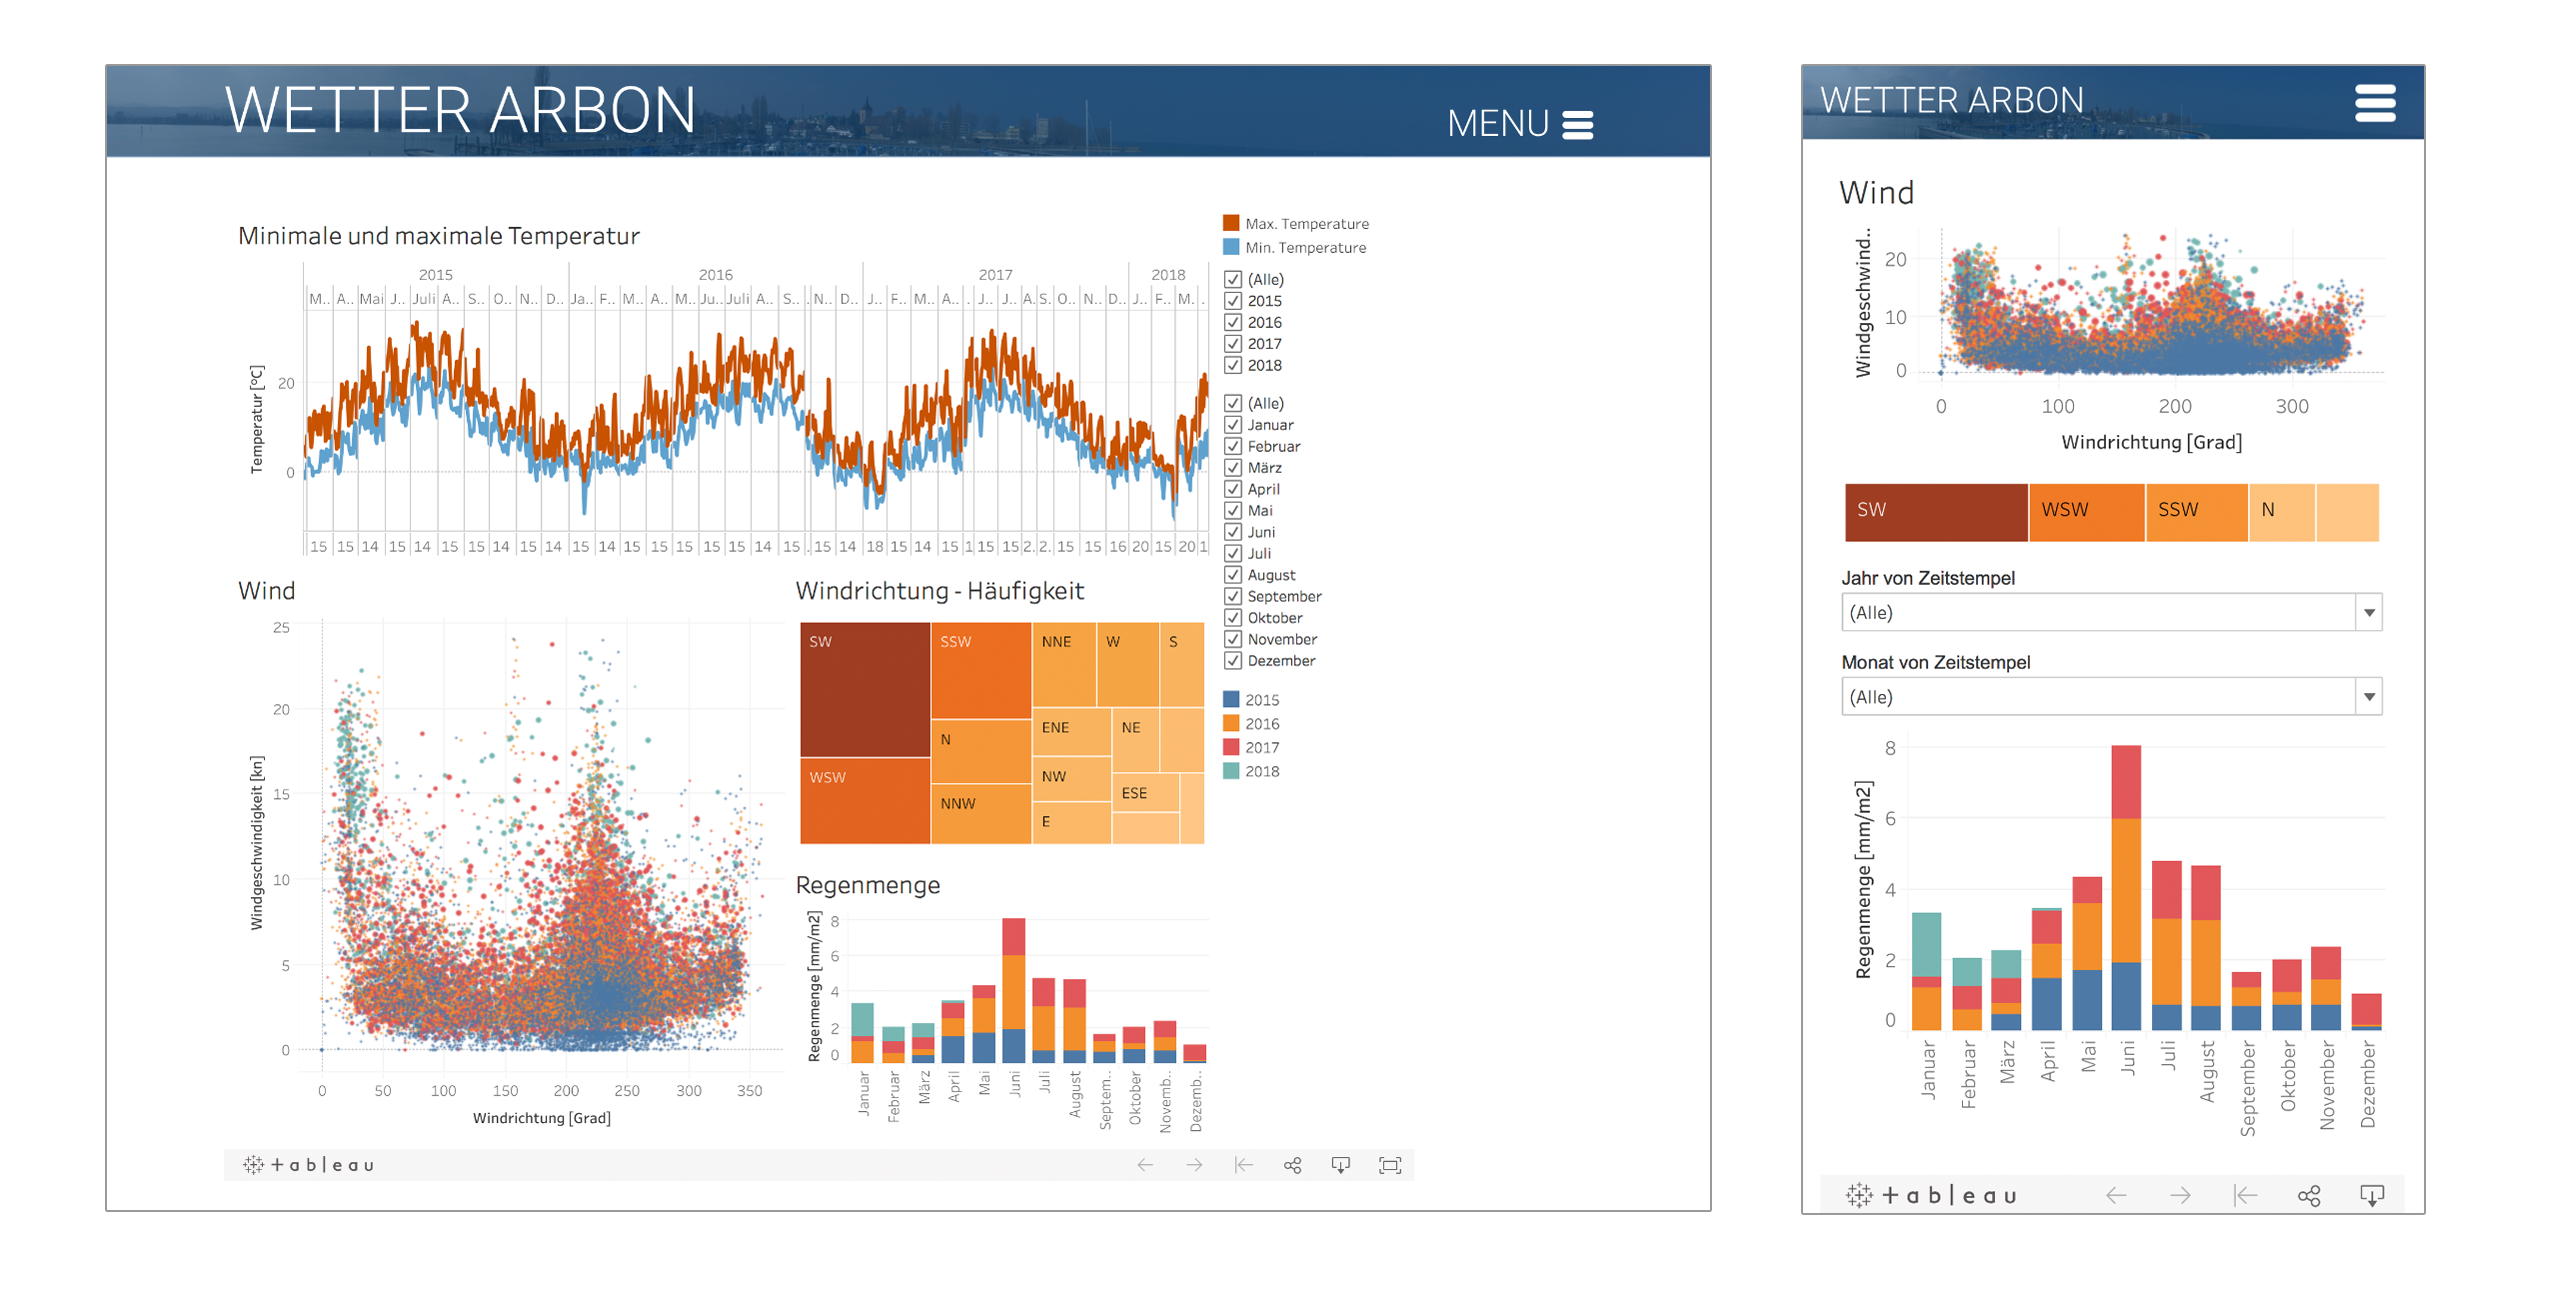
\includegraphics[width=\textwidth-2\fboxsep-2\fboxrule]{img/tableau}}
	\caption{Darstellung der historschen Daten (Desktop und Mobile)}
	\label{img:tableau}
\end{figure}


%Nachteil 2: Nicht responsive -> Workaround nötig
\noindent
Neben den vielen Vorteilen, hat Tableau Pubilc auf ein paar Nachteile. Das Dashbaord kann zwar frei gestaltet werden, ist aber nicht responsive d.h. es passt sich nicht der Bildschirmgrösse an. Das Problem wurd so gelöst, dass zwei verschiedene Dashboard (siehe Abbildung \ref{img:tableau}) erstellt werden. Eines für die Anzeige auf einem grossen Dispaly und eines für die Anzeige auf Mobiltelefonen. Beim Aufruf der Webseite wird die Bildschirmgrösse abgefragt und das entsprechende Dashboard geladen wie in Listing \ref{lst:histViewport} dargestellt.

\begin{lstlisting}[label=lst:histViewport,caption=Auswahl des Dashboards anahnd der Bildschirmgrösse, language=JavaScript, style=htmlcssjs]
(function () {
	var viewportWidth = $(window).width();
	if (viewportWidth > 767) {
		$('#area_3').load('application/php/tableauDesktop.php');
	}
	else {
		$('#area_3').load('application/php/tableauMobile.php');
	}
}());
\end{lstlisting}


% Nachteil 1: Keine direkte Verbindung zur Datenbank
\noindent
Ein weiteren Nachteil von Tableau Public, welches kostenlos ist gegenüber Tableau, welches kostenpflicht ist, ist dass Tableau Public keinen Live-Zugriff auf die Datenbank ermöglicht. Die Daten müssen somit manuell periodisch auf den Tableau Public Server kopiert werden, damit sie im Dashboard verfügbar sind.



\subsubsection{Daten der alten Wetterstation}
Abbildung \ref{img:histAlt} zeigt eine Zusammenfassung der von der alten Wetterstation vorhandenen Daten. Es gibt diverse Messlücken wie z.B. das komplette Jahr 2010 und 2012. Weiter sind z.T. unplausible Grössenordnungen vorhanden wie z.B. die Windgeschwindigkeit von 500, wo nicht klar ist, zu welcher Einheit dieser Angabe gehört. Die Wellenhöhe sieht mehr nach Signalrauschen aus, als nach plausiblem Messwert. Alles in allem sind in diesen Daten nicht viel nützliche Informationen vorhanden. Es wurde deshalb beschlossen auf der Webseite nur die historischen Daten der neuen Wetterstation anzuzeigen. Die Pegeldaten werden in die Grafik, wie in Abschnitt \ref{subsec:pegelhistory} beschrieben integriert.

\begin{figure}[h!]
	\centering
  \fbox{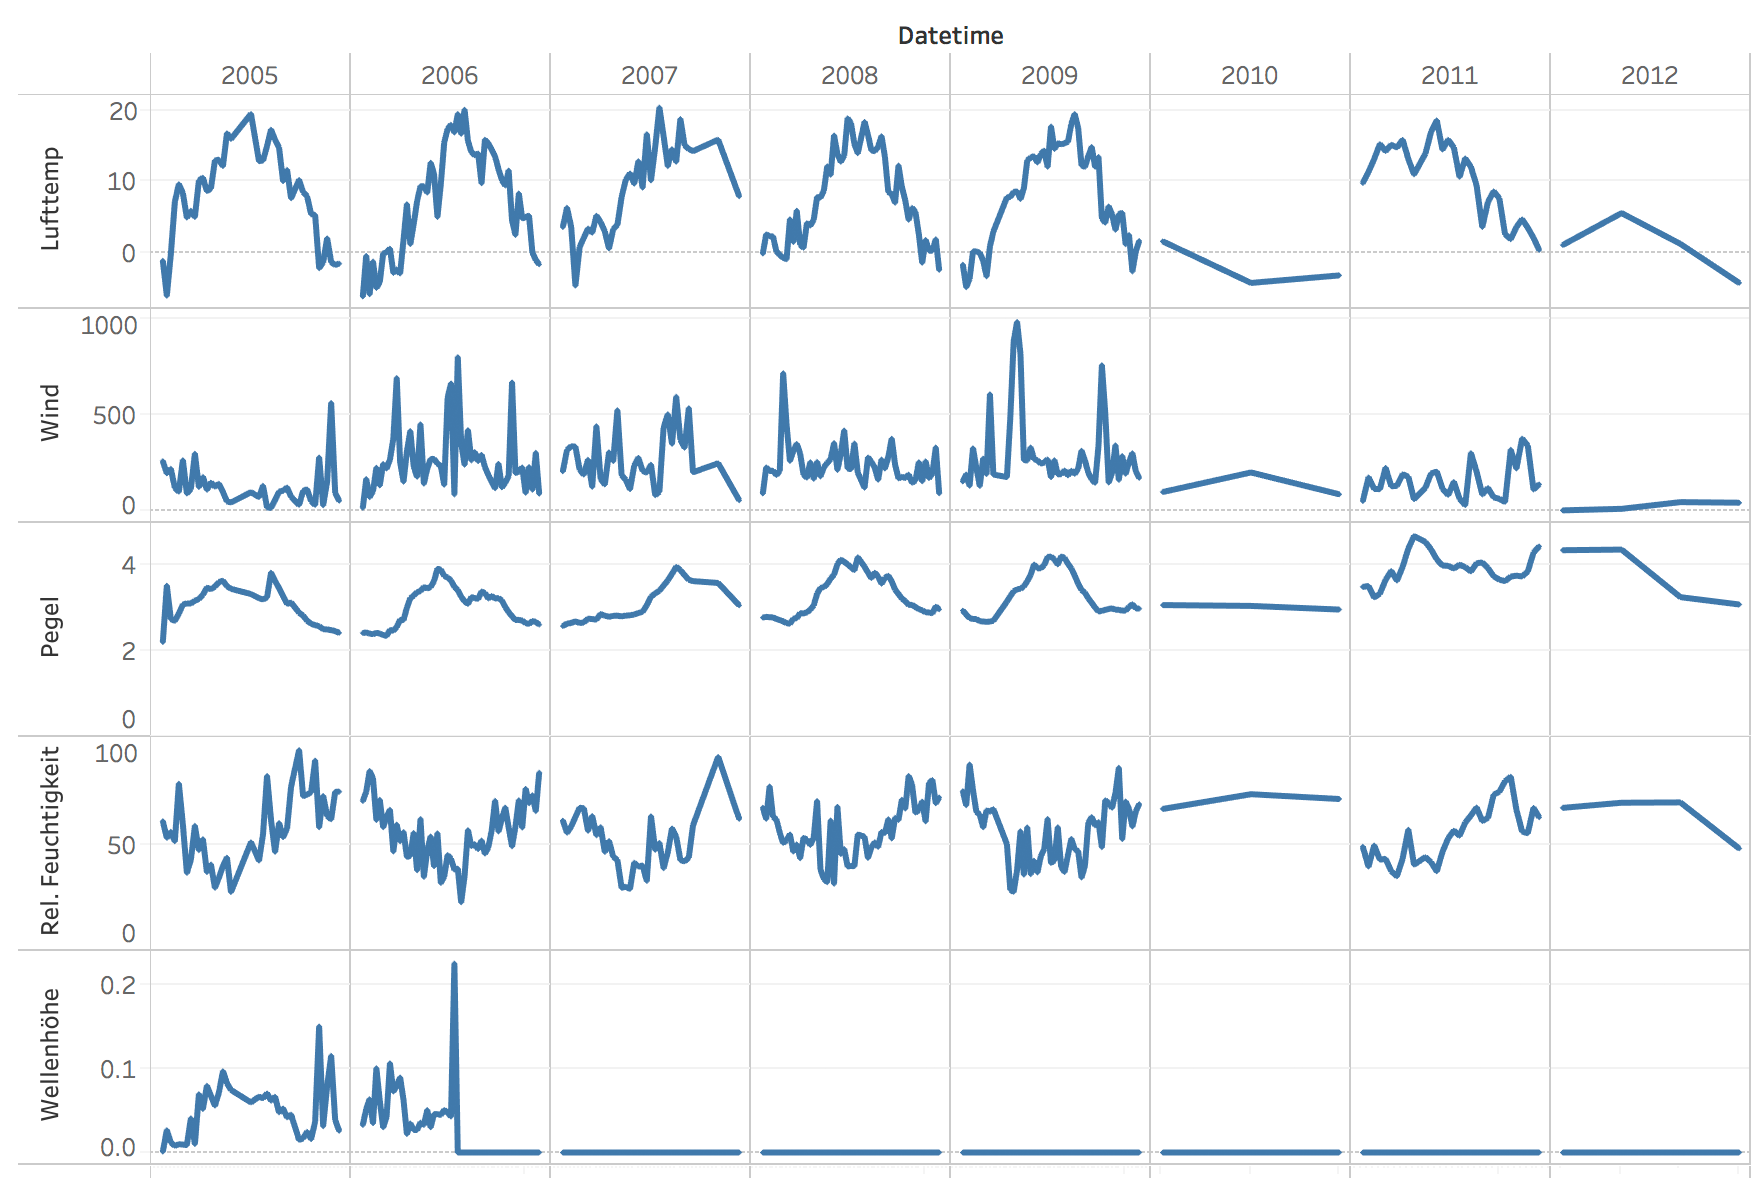
\includegraphics[width=\textwidth-2\fboxsep-2\fboxrule]{img/histAlt}}
	%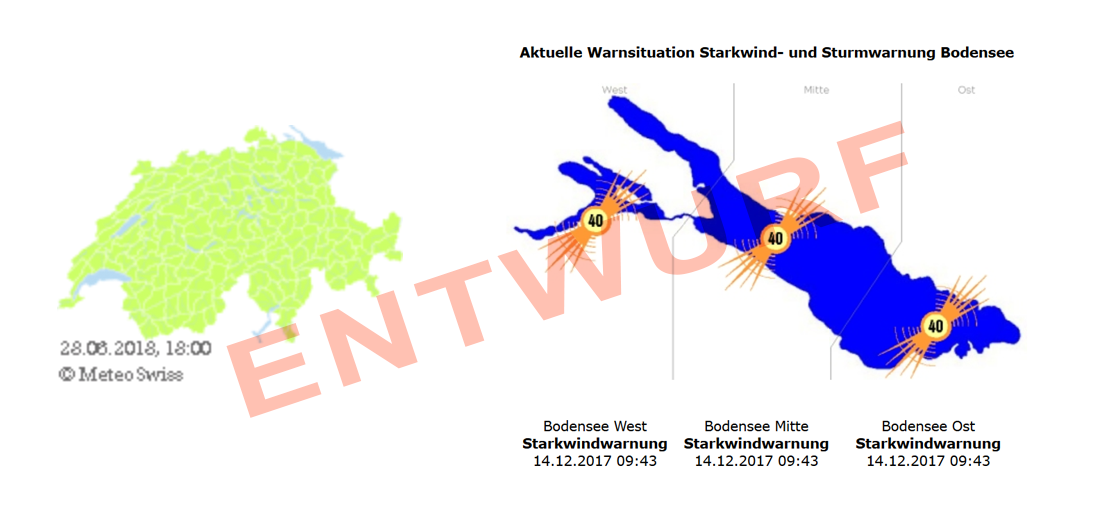
\includegraphics[width=1\linewidth]{img/sturm}
	\caption{Übersicht über die gespeicherten Daten der alten Wetterstation}
	\label{img:histAlt}
\end{figure}



\subsubsection{Pegeldaten 1953 bis 2005}
\label{subsec:pegelhistory}
Auf der Webseite wird der Pegelverlauf der letzten Jahre grafisch dargestellt. Als Grundlage diente u.a. ein Excel-File mit den Pegelständen von 1953 bis 2005. Von der alten Wetterstation liegen die Pegeldaten von 2005 bis 2009 vor und ab 2018 kommen die Messwerte der neuen Wetterstation dazu. Die Darstellung erfolgt analog Abbildung \ref{img:histPegel}. Sämtliche Datenquellen sind in einer gemeinsamen Tabelle in der Datenbank gespeichert. Die grafische Darstellung erfolgt wiederum mit Tableau, was die interaktiven Anzeige mit Filterung der Daten ermöglicht.

\begin{figure}[h!]
	\centering
  \fbox{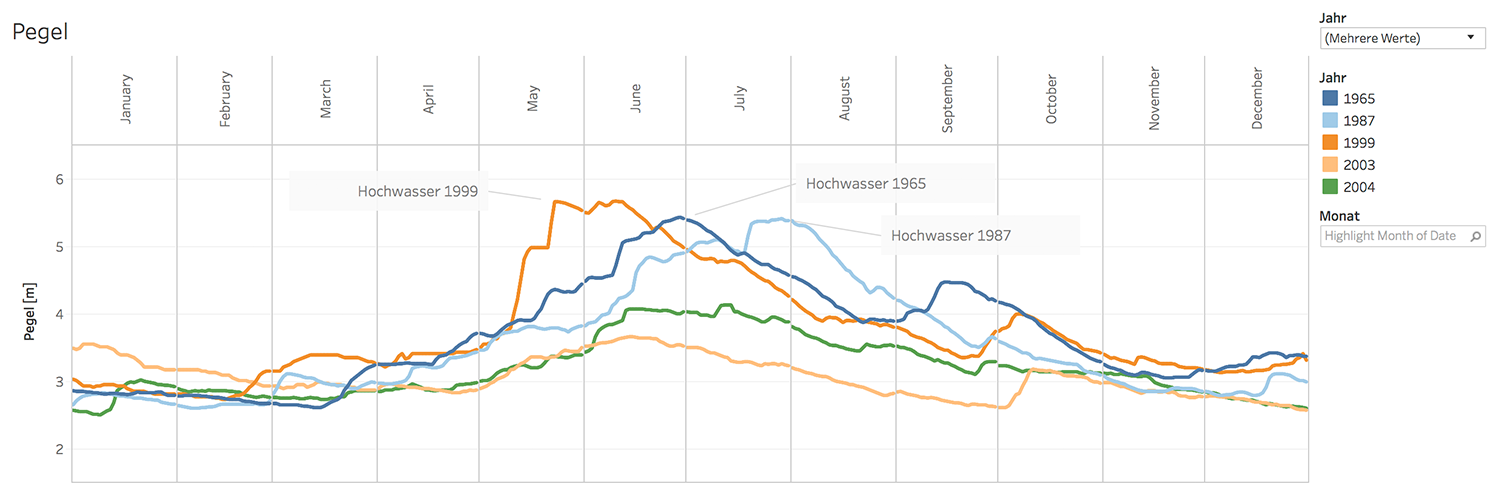
\includegraphics[width=\textwidth-2\fboxsep-2\fboxrule]{img/histPegel}}
	%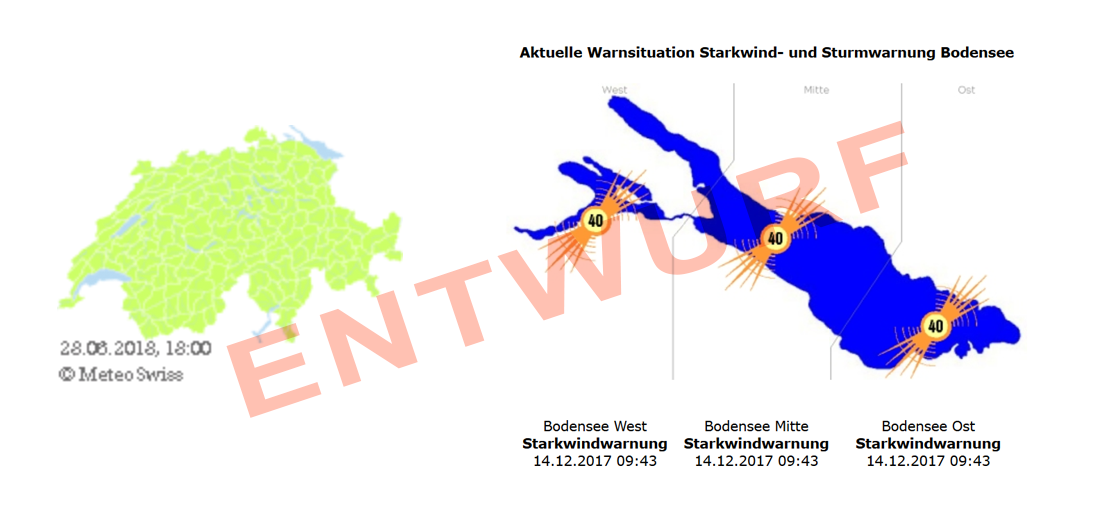
\includegraphics[width=1\linewidth]{img/sturm}
	\caption{Darstellung der historischen Pegelmesswerte}
	\label{img:histPegel}
\end{figure}



%% ############################################################################
%% Unterkapitel
%% ############################################################################
\subsection{Automatische Aktualisierung der Anzeigeelemente}
\Diskussionspunkt{Initial Values beschreiben}\newline
Die Wetterstation erzeugt jede Minute einen Datenbank-Eintrag mit den aktuellen Messwerten. Damit eine geöffnete Webseite immer auf dem aktuellen Stand ist, wird eine poll-Funktion verwendet, die selbständig alle 61 Sekunden von der API die aktuellen Werte abfragt wie in \ref{lst:poll} verkürzt dargestellt. Sobald die JSON-Daten eingetroffen sind, wird die Funktion \textit{updateData} aufgerufen, die wiederum die Anzeigeelemente und Texfelder aktualisiert. Die gesamte Aktualisierung wird asynchron mittels AJAX durchgeführt. Die Seite wird dabei nicht neu geladen, nur die Anzeigewerte. \newline

\begin{lstlisting}[label=lst:poll,caption=Automatische Aktualisierung der Werte, language=JavaScript, style=htmlcssjs]
(function poll() {
        $.get('https://api.wetter-arbon.ch/v1/')
          .done(function(response) {updateData(response);})
          .always(function() {setTimeout(poll, 61000); });
})();

function updateData(res){
        pressure_gauge.refresh(res.v1.data.pressure.value);
        $("#cwassertemp1m") = res.v1.data.watertemperature1m.value;
        ...
}
\end{lstlisting}


%% ############################################################################
%% Unterkapitel
%% ############################################################################
\subsection{Barrierefreier Zugang}
Die Wetterstation und ihre Webseite ist eine Dienstleistung der Stadt Arbon. Sie gehört der Bevölkerung und soll deshalb für möglichst alle zugänglich sein. Sowohl die \flqq Web Content Accessibility Guidelines\frqq\footnote{ \url{https://www.w3.org/TR/2008/REC-WCAG20-20081211/}} des W3C-Konsortiums, als auch die deutsche \flqq  Barrierefreie-Informationstechnik-Verordnung\frqq\footnote{ \url{https://www.gesetze-im-internet.de/bitv_2_0/BJNR184300011.html}} bieten diverse Inputs, wie die Bedienbarkeit und somit Zugänglichkeit einer Webseite verbesserte werden kann. Von einer verbesserten Zugänglichkeit profitieren nicht nur Menschen mit Einschränkungen. Es geht darum, die Webseite so zu gestalten, dass sie möglichst für alle Benutzergruppen zugänglich ist. Eine von Microsoft beauftragte Studie~\cite{ForresterResearch2004E:Abilities} der \flqq Forrester Research Inc.\frqq schätzt, dass über 60 Prozent aller Computernutzer von Barrierefreiheit profitieren können und gemäss \flqq Interface Design\frqq ~\cite{ThesmannStephan2016ID:U} wird Barrierefreiheit bald Standard sein.

\noindent
Die aktuellen Web Content Accessibility Guidelines\footnote{\url{https://www.w3.org/TR/WCAG20/}} fordern die Einhaltung von vier Designprinzipien, welche in gesamthaft zwölf Richtlinien genauer spezifiziert sind.

\begin{itemize}
\item Designprinzip 1: wahrnehmbar
\item Designprinzip 2: bedienbar
\item Designprinzip 3: verständlich
\item Designprinzip 4: robust
\end{itemize}

\noindent
Aus den Richtlinien wurden diejenigen Anforderungen ausgewählt, die auf die Webseite der Wetterstation zutreffen und die im Rahmen des CMS umsetzbar sind. Alle relevanten Anforderungen und deren Umsetzung werden im Folgenden beschrieben.

\subsubsection{Wahrnehmbarkeit}
% Richtlinie 1.1
\href{https://www.w3.org/Translations/WCAG20-de/#text-equiv}{Richtlinie 1.1} fordert, dass für alle Nicht-Text-Inhalte eine Textalternative zur Verfügung steht. Auf der Webseite mit den aktuellen Messwerten gibt es drei Typen von Nicht-Text-Inhalten: Gauges, Icons und Graphen. Bei den Gauges und Graphen werden fertige javascript-Bibliotheken verwendet. Diese stellen leider keine Möglichkeit zur Verfügung einen Alternativtext hinzuzufügen. Für die Icons, welche als \textit{img} gekennzeichnet sind, wurde das \textit{alt}-Attribut ausgefüllt, wie in Listing \ref{lst:altImg} beispielhaft dargestellt.

\begin{lstlisting}[label=lst:altImg,caption=Alternativtext für Icons, language=HTML5, style=htmlcssjs]
<img src="img/wi-humidity.svg" alt="Icon eines Barometers">
\end{lstlisting}

Wie die verwendeten javascript-Bibliotheken, bietet auch Tableau, mit welchem die interaktive Darstellung der historischen Daten erfolgt, keine Möglichkeit die Visualisierung als Text darzustellen. \newline

% Richtlinie 1.3
\noindent
\href{https://www.w3.org/Translations/WCAG20-de/#text-equiv}{Richtlinie 1.3} fordert, dass die Struktur d.h. die Zusammenhänge und die Bedeutung einer Webseite unabhängig der Formatierung erhalten bleiben. Man spricht hier auch von \textit{semantischem} Web.

Auf der Webseite wurde eine hierarchische Struktur implementiert, siehe Abbildung \ref{img:semWeb}. Die Hierarchiestufe wird einerseits erkennbar durch die Stufe der Überschriften (h1...h3) und andererseite durch die Bezeichnung der verschiedenen Inhaltsblöcke. Auf der Webseite sind zwei Hauptblöcke erkennbar, sogenannte \textit{Sektionen}. Eine Sektion beinhaltet die aktuellen Messwerte und die andere die Messdatenverläufe. Eine \href{https://www.w3.org/TR/2011/WD-html5-20110525/sections.html#the-section-element}{\textit{Sektion}} ist eine thematische Gruppierung von Elementen. Innerhalb der Sektion gibt es mehrere \href{https://www.w3.org/TR/2011/WD-html5-20110525/sections.html#the-article-element}{\textit{Artikel}}, welche einen unabhängigen Informationsblock darstellen.

\begin{figure}[h!]
	\centering
  \fbox{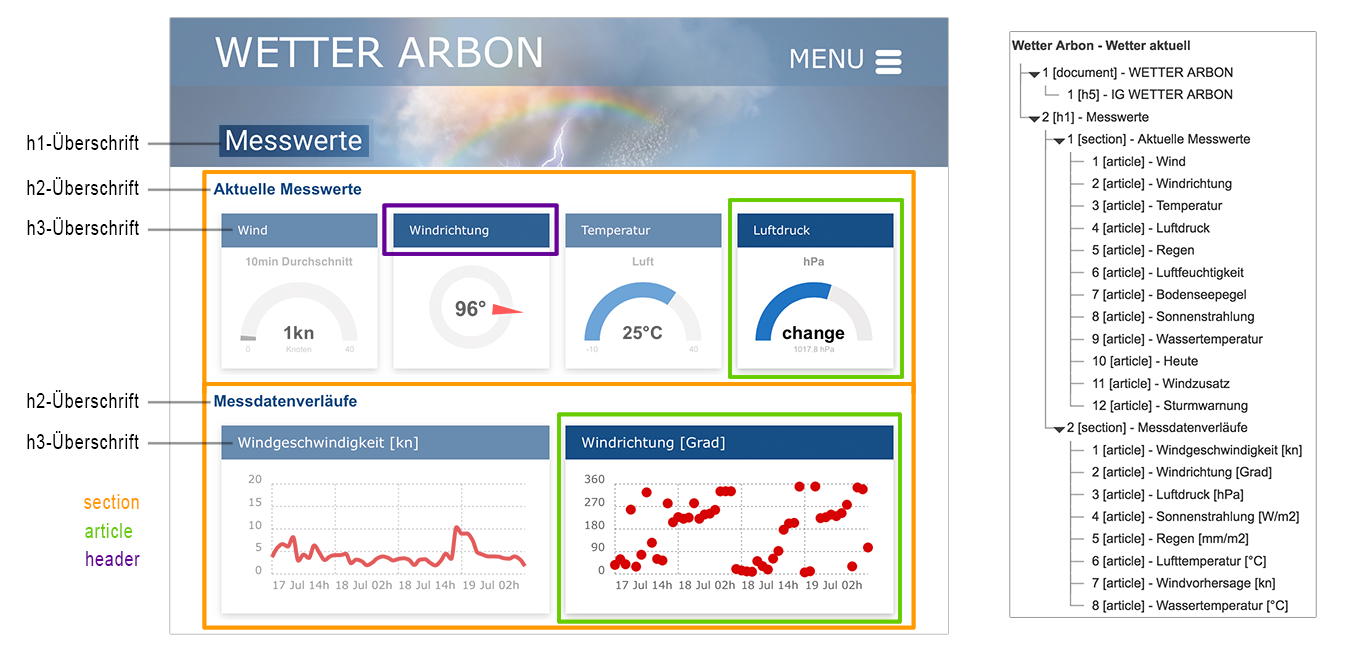
\includegraphics[width=\textwidth-2\fboxsep-2\fboxrule]{img/semWeb}}
	%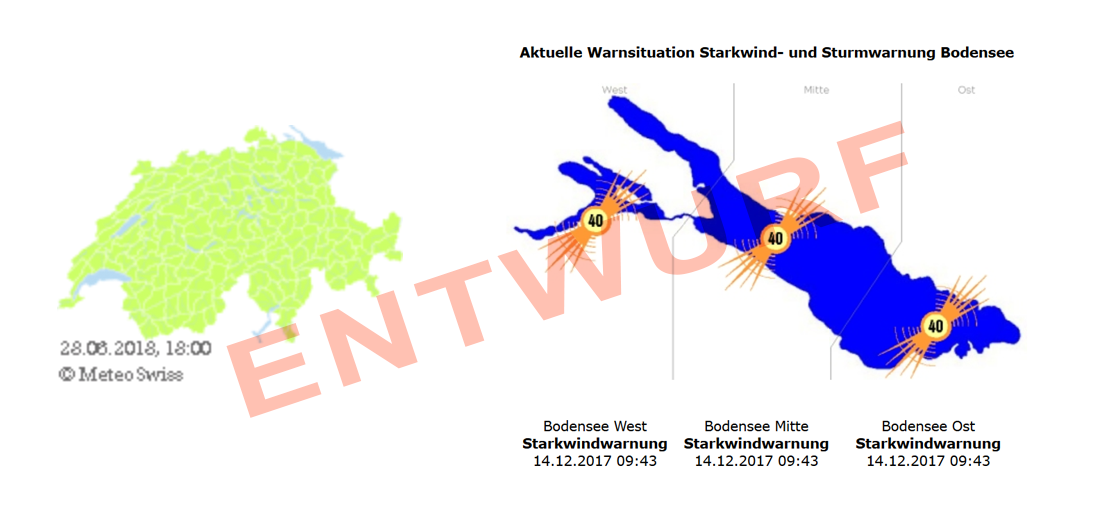
\includegraphics[width=1\linewidth]{img/sturm}
	\caption{Umsetzung der semantisches Web-Anforderung}
	\label{img:semWeb}
\end{figure}

% Richtlinie 1.4
\noindent
\href{https://www.w3.org/Translations/WCAG20-de/#visual-audio-contrast}{Richtlinie 1.4} fordert, dass die visuelle Darstellung von Text ein Kontrastverhältnis von mindestens 4,5:1 hat. Zudem muss es möglich sein die Textgrösse um bis zu 200 Prozent zu erhöhen, ohne dass dabei Inhalt oder Funktionalität verloren geht. Um diese Anforderung zu Überprüfen wurde das Firefox-Plugin \textit{tota11y}\footnote{\url{http://khan.github.io/tota11y/}} verwendet. Das Plugin ermöglicht es auf einfache Weise zu überprüfen ob die Webseite die Barrierefrei-Bediungungen erfüllt. Die Kontrastverhältnisse liegen gemäss diesem Tool zwischen 5.75 und 12.63 und sind somit in Ordnung. Da die gesamte Webseite responsive ist, stellt die Vergrösserung auf 200\% kein Problem dar.


\subsubsection{Bedienbarkeit}
\href{https://www.w3.org/Translations/WCAG20-de/#keyboard-operation}{Richtlinie 2.1} fordert, dass alle Funktionen über eine Tastaturschnittstelle bedienbar sind und das die Tastaturfokusanzeige sichtbar ist.
Da es sich bei der Webseite der Wetterstation primär um eine Anzeige handelt, ist dieses Anforderung nur für das Eingabeformular des Benachrichtiungsservice, siehe Kapitel \ref{notifications}, relevant. Dieses ist problemlos mittels Tastatur bedienbar. \newline

\noindent
\href{https://www.w3.org/Translations/WCAG20-de/#navigation-mechanisms}{Richtlinie 2.4} fordert, dass Webseiten einen zweckbeschreibenden Titel aufweisen und dass Zwischentitel den Inhalt und Zweck des entsprechenden Blocks beschreiben. Wie in Abbildung \ref{img:semWeb} wurde besitzt die Webseite sowhol einen Seitentitel, als auch Zwischentitel.


\subsubsection{Verständlichkeit}
\href{https://www.w3.org/Translations/WCAG20-de/#minimize-error}{Richtlinie 3.3} fordert, dass Eingabefehler automatisch erkannt und dem Benutzer angezeigt werden. Zudem sind Korrekturvorschläge anzuzeigen. Diese Anforderung betrifft insbesondere das Formular des Benachrichtigungsservices, welcher in Kapitel \ref{notifications} beschrieben wird. Diese Anforderung wird erfüllt, wie in Abbildung \ref{img:notificationFE} rechts, dargestellt.


\subsubsection{Robustheit}
\href{https://www.w3.org/Translations/WCAG20-de/#ensure-compat}{Richtlinie 4.1} fordert, dass Inhalten, die mit Hilfe von Markup-Sprachen implementiert wurden,  vollständige Start- und End-Tags haben. Es sind keine doppelten Attribute vorhanden und alle IDs sind eindeutig. Diese Anforderung wurde ebenfalls vollständig umgesetzt. Beispielhaft ist dies in Listing \ref{lst:gaugeHTML} ersichtlich.
